\documentclass[twoside]{book}

% Packages required by doxygen
\usepackage{fixltx2e}
\usepackage{calc}
\usepackage{doxygen}
\usepackage[export]{adjustbox} % also loads graphicx
\usepackage{graphicx}
\usepackage[utf8]{inputenc}
\usepackage{makeidx}
\usepackage{multicol}
\usepackage{multirow}
\PassOptionsToPackage{warn}{textcomp}
\usepackage{textcomp}
\usepackage[nointegrals]{wasysym}
\usepackage[table]{xcolor}

% Font selection
\usepackage[T1]{fontenc}
\usepackage[scaled=.90]{helvet}
\usepackage{courier}
\usepackage{amssymb}
\usepackage{sectsty}
\renewcommand{\familydefault}{\sfdefault}
\allsectionsfont{%
  \fontseries{bc}\selectfont%
  \color{darkgray}%
}
\renewcommand{\DoxyLabelFont}{%
  \fontseries{bc}\selectfont%
  \color{darkgray}%
}
\newcommand{\+}{\discretionary{\mbox{\scriptsize$\hookleftarrow$}}{}{}}

% Page & text layout
\usepackage{geometry}
\geometry{%
  a4paper,%
  top=2.5cm,%
  bottom=2.5cm,%
  left=2.5cm,%
  right=2.5cm%
}
\tolerance=750
\hfuzz=15pt
\hbadness=750
\setlength{\emergencystretch}{15pt}
\setlength{\parindent}{0cm}
\setlength{\parskip}{3ex plus 2ex minus 2ex}
\makeatletter
\renewcommand{\paragraph}{%
  \@startsection{paragraph}{4}{0ex}{-1.0ex}{1.0ex}{%
    \normalfont\normalsize\bfseries\SS@parafont%
  }%
}
\renewcommand{\subparagraph}{%
  \@startsection{subparagraph}{5}{0ex}{-1.0ex}{1.0ex}{%
    \normalfont\normalsize\bfseries\SS@subparafont%
  }%
}
\makeatother

% Headers & footers
\usepackage{fancyhdr}
\pagestyle{fancyplain}
\fancyhead[LE]{\fancyplain{}{\bfseries\thepage}}
\fancyhead[CE]{\fancyplain{}{}}
\fancyhead[RE]{\fancyplain{}{\bfseries\leftmark}}
\fancyhead[LO]{\fancyplain{}{\bfseries\rightmark}}
\fancyhead[CO]{\fancyplain{}{}}
\fancyhead[RO]{\fancyplain{}{\bfseries\thepage}}
\fancyfoot[LE]{\fancyplain{}{}}
\fancyfoot[CE]{\fancyplain{}{}}
\fancyfoot[RE]{\fancyplain{}{\bfseries\scriptsize Generated by Doxygen }}
\fancyfoot[LO]{\fancyplain{}{\bfseries\scriptsize Generated by Doxygen }}
\fancyfoot[CO]{\fancyplain{}{}}
\fancyfoot[RO]{\fancyplain{}{}}
\renewcommand{\footrulewidth}{0.4pt}
\renewcommand{\chaptermark}[1]{%
  \markboth{#1}{}%
}
\renewcommand{\sectionmark}[1]{%
  \markright{\thesection\ #1}%
}

% Indices & bibliography
\usepackage{natbib}
\usepackage[titles]{tocloft}
\setcounter{tocdepth}{3}
\setcounter{secnumdepth}{5}
\makeindex

% Hyperlinks (required, but should be loaded last)
\usepackage{ifpdf}
\ifpdf
  \usepackage[pdftex,pagebackref=true]{hyperref}
\else
  \usepackage[ps2pdf,pagebackref=true]{hyperref}
\fi
\hypersetup{%
  colorlinks=true,%
  linkcolor=blue,%
  citecolor=blue,%
  unicode%
}

% Custom commands
\newcommand{\clearemptydoublepage}{%
  \newpage{\pagestyle{empty}\cleardoublepage}%
}

\usepackage{caption}
\captionsetup{labelsep=space,justification=centering,font={bf},singlelinecheck=off,skip=4pt,position=top}

%===== C O N T E N T S =====

\begin{document}

% Titlepage & ToC
\hypersetup{pageanchor=false,
             bookmarksnumbered=true,
             pdfencoding=unicode
            }
\pagenumbering{alph}
\begin{titlepage}
\vspace*{7cm}
\begin{center}%
{\Large My Project }\\
\vspace*{1cm}
{\large Generated by Doxygen 1.8.13}\\
\end{center}
\end{titlepage}
\clearemptydoublepage
\pagenumbering{roman}
\tableofcontents
\clearemptydoublepage
\pagenumbering{arabic}
\hypersetup{pageanchor=true}

%--- Begin generated contents ---
\chapter{Namespace Index}
\section{Packages}
Here are the packages with brief descriptions (if available)\+:\begin{DoxyCompactList}
\item\contentsline{section}{\hyperlink{namespacescripts_1_1carla__plugin}{scripts.\+carla\+\_\+plugin} \\*Does things }{\pageref{namespacescripts_1_1carla__plugin}}{}
\item\contentsline{section}{\hyperlink{namespacescripts_1_1osu__modules_1_1dynamics_1_1av}{scripts.\+osu\+\_\+modules.\+dynamics.\+av} }{\pageref{namespacescripts_1_1osu__modules_1_1dynamics_1_1av}}{}
\item\contentsline{section}{\hyperlink{namespacescripts_1_1osu__modules_1_1dynamics_1_1vel__control}{scripts.\+osu\+\_\+modules.\+dynamics.\+vel\+\_\+control} }{\pageref{namespacescripts_1_1osu__modules_1_1dynamics_1_1vel__control}}{}
\item\contentsline{section}{\hyperlink{namespacescripts_1_1osu__modules_1_1nav_1_1navigator}{scripts.\+osu\+\_\+modules.\+nav.\+navigator} \\*Does things }{\pageref{namespacescripts_1_1osu__modules_1_1nav_1_1navigator}}{}
\item\contentsline{section}{\hyperlink{namespacescripts_1_1osu__modules_1_1nav_1_1planner}{scripts.\+osu\+\_\+modules.\+nav.\+planner} \\*Does things }{\pageref{namespacescripts_1_1osu__modules_1_1nav_1_1planner}}{}
\item\contentsline{section}{\hyperlink{namespacescripts_1_1osu__modules_1_1tools_1_1robotic__helper}{scripts.\+osu\+\_\+modules.\+tools.\+robotic\+\_\+helper} \\*Does things }{\pageref{namespacescripts_1_1osu__modules_1_1tools_1_1robotic__helper}}{}
\end{DoxyCompactList}

\chapter{Hierarchical Index}
\section{Class Hierarchy}
This inheritance list is sorted roughly, but not completely, alphabetically\+:\begin{DoxyCompactList}
\item \contentsline{section}{test\+\_\+\+A\+V\+\_\+control.\+Input\+Message}{\pageref{classtest__AV__control_1_1InputMessage}}{}
\item object\begin{DoxyCompactList}
\item \contentsline{section}{scripts.\+agents.\+navigation.\+agent.\+Agent}{\pageref{classscripts_1_1agents_1_1navigation_1_1agent_1_1Agent}}{}
\begin{DoxyCompactList}
\item \contentsline{section}{scripts.\+agents.\+navigation.\+basic\+\_\+agent.\+Basic\+Agent}{\pageref{classscripts_1_1agents_1_1navigation_1_1basic__agent_1_1BasicAgent}}{}
\item \contentsline{section}{scripts.\+agents.\+navigation.\+roaming\+\_\+agent.\+Roaming\+Agent}{\pageref{classscripts_1_1agents_1_1navigation_1_1roaming__agent_1_1RoamingAgent}}{}
\end{DoxyCompactList}
\item \contentsline{section}{scripts.\+agents.\+navigation.\+global\+\_\+route\+\_\+planner.\+Global\+Route\+Planner}{\pageref{classscripts_1_1agents_1_1navigation_1_1global__route__planner_1_1GlobalRoutePlanner}}{}
\item \contentsline{section}{scripts.\+agents.\+navigation.\+global\+\_\+route\+\_\+planner\+\_\+dao.\+Global\+Route\+Planner\+D\+AO}{\pageref{classscripts_1_1agents_1_1navigation_1_1global__route__planner__dao_1_1GlobalRoutePlannerDAO}}{}
\item \contentsline{section}{scripts.\+agents.\+navigation.\+local\+\_\+planner.\+Local\+Planner}{\pageref{classscripts_1_1agents_1_1navigation_1_1local__planner_1_1LocalPlanner}}{}
\item \contentsline{section}{scripts.\+osu\+\_\+modules.\+dynamics.\+vel\+\_\+control.\+Vehicle\+Velocity\+Control}{\pageref{classscripts_1_1osu__modules_1_1dynamics_1_1vel__control_1_1VehicleVelocityControl}}{}
\item \contentsline{section}{scripts.\+osu\+\_\+modules.\+nav.\+navigator.\+Nav}{\pageref{classscripts_1_1osu__modules_1_1nav_1_1navigator_1_1Nav}}{}
\begin{DoxyCompactList}
\item \contentsline{section}{scripts.\+osu\+\_\+modules.\+nav.\+planner.\+Plan}{\pageref{classscripts_1_1osu__modules_1_1nav_1_1planner_1_1Plan}}{}
\begin{DoxyCompactList}
\item \contentsline{section}{scripts.\+osu\+\_\+modules.\+nav.\+roamer.\+Roamer}{\pageref{classscripts_1_1osu__modules_1_1nav_1_1roamer_1_1Roamer}}{}
\begin{DoxyCompactList}
\item \contentsline{section}{scripts.\+osu\+\_\+modules.\+dynamics.\+av.\+AV}{\pageref{classscripts_1_1osu__modules_1_1dynamics_1_1av_1_1AV}}{}
\end{DoxyCompactList}
\end{DoxyCompactList}
\end{DoxyCompactList}
\item \contentsline{section}{scripts.\+osu\+\_\+modules.\+tools.\+robotic\+\_\+helper.\+Robotic\+Helper}{\pageref{classscripts_1_1osu__modules_1_1tools_1_1robotic__helper_1_1RoboticHelper}}{}
\end{DoxyCompactList}
\item \contentsline{section}{test\+\_\+\+A\+V\+\_\+control.\+Output\+Message}{\pageref{classtest__AV__control_1_1OutputMessage}}{}
\item \contentsline{section}{scripts.\+agents.\+navigation.\+controller.\+P\+I\+D\+Lateral\+Controller}{\pageref{classscripts_1_1agents_1_1navigation_1_1controller_1_1PIDLateralController}}{}
\item \contentsline{section}{scripts.\+agents.\+navigation.\+controller.\+P\+I\+D\+Longitudinal\+Controller}{\pageref{classscripts_1_1agents_1_1navigation_1_1controller_1_1PIDLongitudinalController}}{}
\item \contentsline{section}{test\+\_\+\+A\+V\+\_\+control.\+R\+O\+S\+Wrapper\+For\+AV}{\pageref{classtest__AV__control_1_1ROSWrapperForAV}}{}
\item \contentsline{section}{scripts.\+agents.\+navigation.\+controller.\+Vehicle\+P\+I\+D\+Controller}{\pageref{classscripts_1_1agents_1_1navigation_1_1controller_1_1VehiclePIDController}}{}
\item Agent\begin{DoxyCompactList}
\item \contentsline{section}{test\+\_\+\+A\+V\+\_\+control.\+AV}{\pageref{classtest__AV__control_1_1AV}}{}
\end{DoxyCompactList}
\item Enum\begin{DoxyCompactList}
\item \contentsline{section}{scripts.\+agents.\+navigation.\+agent.\+Agent\+State}{\pageref{classscripts_1_1agents_1_1navigation_1_1agent_1_1AgentState}}{}
\item \contentsline{section}{scripts.\+agents.\+navigation.\+local\+\_\+planner.\+Road\+Option}{\pageref{classscripts_1_1agents_1_1navigation_1_1local__planner_1_1RoadOption}}{}
\item \contentsline{section}{scripts.\+osu\+\_\+modules.\+nav.\+planner.\+Road\+Option}{\pageref{classscripts_1_1osu__modules_1_1nav_1_1planner_1_1RoadOption}}{}
\item \contentsline{section}{scripts.\+osu\+\_\+modules.\+nav.\+roamer.\+\_\+\+Agent\+State}{\pageref{classscripts_1_1osu__modules_1_1nav_1_1roamer_1_1__AgentState}}{}
\end{DoxyCompactList}
\end{DoxyCompactList}

\chapter{Class Index}
\section{Class List}
Here are the classes, structs, unions and interfaces with brief descriptions\+:\begin{DoxyCompactList}
\item\contentsline{section}{\hyperlink{classscripts_1_1osu__modules_1_1nav_1_1roamer_1_1__AgentState}{scripts.\+osu\+\_\+modules.\+nav.\+roamer.\+\_\+\+Agent\+State} }{\pageref{classscripts_1_1osu__modules_1_1nav_1_1roamer_1_1__AgentState}}{}
\item\contentsline{section}{\hyperlink{classscripts_1_1agents_1_1navigation_1_1agent_1_1Agent}{scripts.\+agents.\+navigation.\+agent.\+Agent} }{\pageref{classscripts_1_1agents_1_1navigation_1_1agent_1_1Agent}}{}
\item\contentsline{section}{\hyperlink{classscripts_1_1agents_1_1navigation_1_1agent_1_1AgentState}{scripts.\+agents.\+navigation.\+agent.\+Agent\+State} }{\pageref{classscripts_1_1agents_1_1navigation_1_1agent_1_1AgentState}}{}
\item\contentsline{section}{\hyperlink{classtest__AV__control_1_1AV}{test\+\_\+\+A\+V\+\_\+control.\+AV} \\*\hyperlink{classtest__AV__control_1_1AV}{AV} class }{\pageref{classtest__AV__control_1_1AV}}{}
\item\contentsline{section}{\hyperlink{classscripts_1_1osu__modules_1_1dynamics_1_1av_1_1AV}{scripts.\+osu\+\_\+modules.\+dynamics.\+av.\+AV} }{\pageref{classscripts_1_1osu__modules_1_1dynamics_1_1av_1_1AV}}{}
\item\contentsline{section}{\hyperlink{classscripts_1_1agents_1_1navigation_1_1basic__agent_1_1BasicAgent}{scripts.\+agents.\+navigation.\+basic\+\_\+agent.\+Basic\+Agent} }{\pageref{classscripts_1_1agents_1_1navigation_1_1basic__agent_1_1BasicAgent}}{}
\item\contentsline{section}{\hyperlink{classscripts_1_1agents_1_1navigation_1_1global__route__planner_1_1GlobalRoutePlanner}{scripts.\+agents.\+navigation.\+global\+\_\+route\+\_\+planner.\+Global\+Route\+Planner} }{\pageref{classscripts_1_1agents_1_1navigation_1_1global__route__planner_1_1GlobalRoutePlanner}}{}
\item\contentsline{section}{\hyperlink{classscripts_1_1agents_1_1navigation_1_1global__route__planner__dao_1_1GlobalRoutePlannerDAO}{scripts.\+agents.\+navigation.\+global\+\_\+route\+\_\+planner\+\_\+dao.\+Global\+Route\+Planner\+D\+AO} }{\pageref{classscripts_1_1agents_1_1navigation_1_1global__route__planner__dao_1_1GlobalRoutePlannerDAO}}{}
\item\contentsline{section}{\hyperlink{classtest__AV__control_1_1InputMessage}{test\+\_\+\+A\+V\+\_\+control.\+Input\+Message} }{\pageref{classtest__AV__control_1_1InputMessage}}{}
\item\contentsline{section}{\hyperlink{classscripts_1_1agents_1_1navigation_1_1local__planner_1_1LocalPlanner}{scripts.\+agents.\+navigation.\+local\+\_\+planner.\+Local\+Planner} }{\pageref{classscripts_1_1agents_1_1navigation_1_1local__planner_1_1LocalPlanner}}{}
\item\contentsline{section}{\hyperlink{classscripts_1_1osu__modules_1_1nav_1_1navigator_1_1Nav}{scripts.\+osu\+\_\+modules.\+nav.\+navigator.\+Nav} }{\pageref{classscripts_1_1osu__modules_1_1nav_1_1navigator_1_1Nav}}{}
\item\contentsline{section}{\hyperlink{classtest__AV__control_1_1OutputMessage}{test\+\_\+\+A\+V\+\_\+control.\+Output\+Message} }{\pageref{classtest__AV__control_1_1OutputMessage}}{}
\item\contentsline{section}{\hyperlink{classscripts_1_1agents_1_1navigation_1_1controller_1_1PIDLateralController}{scripts.\+agents.\+navigation.\+controller.\+P\+I\+D\+Lateral\+Controller} }{\pageref{classscripts_1_1agents_1_1navigation_1_1controller_1_1PIDLateralController}}{}
\item\contentsline{section}{\hyperlink{classscripts_1_1agents_1_1navigation_1_1controller_1_1PIDLongitudinalController}{scripts.\+agents.\+navigation.\+controller.\+P\+I\+D\+Longitudinal\+Controller} }{\pageref{classscripts_1_1agents_1_1navigation_1_1controller_1_1PIDLongitudinalController}}{}
\item\contentsline{section}{\hyperlink{classscripts_1_1osu__modules_1_1nav_1_1planner_1_1Plan}{scripts.\+osu\+\_\+modules.\+nav.\+planner.\+Plan} }{\pageref{classscripts_1_1osu__modules_1_1nav_1_1planner_1_1Plan}}{}
\item\contentsline{section}{\hyperlink{classscripts_1_1agents_1_1navigation_1_1local__planner_1_1RoadOption}{scripts.\+agents.\+navigation.\+local\+\_\+planner.\+Road\+Option} }{\pageref{classscripts_1_1agents_1_1navigation_1_1local__planner_1_1RoadOption}}{}
\item\contentsline{section}{\hyperlink{classscripts_1_1osu__modules_1_1nav_1_1planner_1_1RoadOption}{scripts.\+osu\+\_\+modules.\+nav.\+planner.\+Road\+Option} }{\pageref{classscripts_1_1osu__modules_1_1nav_1_1planner_1_1RoadOption}}{}
\item\contentsline{section}{\hyperlink{classscripts_1_1osu__modules_1_1nav_1_1roamer_1_1Roamer}{scripts.\+osu\+\_\+modules.\+nav.\+roamer.\+Roamer} }{\pageref{classscripts_1_1osu__modules_1_1nav_1_1roamer_1_1Roamer}}{}
\item\contentsline{section}{\hyperlink{classscripts_1_1agents_1_1navigation_1_1roaming__agent_1_1RoamingAgent}{scripts.\+agents.\+navigation.\+roaming\+\_\+agent.\+Roaming\+Agent} }{\pageref{classscripts_1_1agents_1_1navigation_1_1roaming__agent_1_1RoamingAgent}}{}
\item\contentsline{section}{\hyperlink{classscripts_1_1osu__modules_1_1tools_1_1robotic__helper_1_1RoboticHelper}{scripts.\+osu\+\_\+modules.\+tools.\+robotic\+\_\+helper.\+Robotic\+Helper} }{\pageref{classscripts_1_1osu__modules_1_1tools_1_1robotic__helper_1_1RoboticHelper}}{}
\item\contentsline{section}{\hyperlink{classtest__AV__control_1_1ROSWrapperForAV}{test\+\_\+\+A\+V\+\_\+control.\+R\+O\+S\+Wrapper\+For\+AV} }{\pageref{classtest__AV__control_1_1ROSWrapperForAV}}{}
\item\contentsline{section}{\hyperlink{classscripts_1_1agents_1_1navigation_1_1controller_1_1VehiclePIDController}{scripts.\+agents.\+navigation.\+controller.\+Vehicle\+P\+I\+D\+Controller} }{\pageref{classscripts_1_1agents_1_1navigation_1_1controller_1_1VehiclePIDController}}{}
\item\contentsline{section}{\hyperlink{classscripts_1_1osu__modules_1_1dynamics_1_1vel__control_1_1VehicleVelocityControl}{scripts.\+osu\+\_\+modules.\+dynamics.\+vel\+\_\+control.\+Vehicle\+Velocity\+Control} }{\pageref{classscripts_1_1osu__modules_1_1dynamics_1_1vel__control_1_1VehicleVelocityControl}}{}
\end{DoxyCompactList}

\chapter{Namespace Documentation}
\hypertarget{namespacescripts_1_1carla__plugin}{}\section{scripts.\+carla\+\_\+plugin Namespace Reference}
\label{namespacescripts_1_1carla__plugin}\index{scripts.\+carla\+\_\+plugin@{scripts.\+carla\+\_\+plugin}}


does things  


\subsection*{Functions}
\begin{DoxyCompactItemize}
\item 
def \hyperlink{namespacescripts_1_1carla__plugin_a23dd1a2cff4ea023f7d9a2ebad524014}{loop} (car)
\item 
def \hyperlink{namespacescripts_1_1carla__plugin_a779dc6d947f91025ecee9c1a340c98de}{exit\+\_\+handler} (signum, frame)
\item 
def \hyperlink{namespacescripts_1_1carla__plugin_a6d9a5090669749d928df2f9af020588f}{test\+\_\+velocity\+\_\+process} (car)
\begin{DoxyCompactList}\small\item\em function used for testing \end{DoxyCompactList}\end{DoxyCompactItemize}
\subsection*{Variables}
\begin{DoxyCompactItemize}
\item 
\mbox{\Hypertarget{namespacescripts_1_1carla__plugin_a9147b8d018233e8bb5995067aebe955e}\label{namespacescripts_1_1carla__plugin_a9147b8d018233e8bb5995067aebe955e}} 
{\bfseries A\+R\+G\+P\+A\+R\+S\+ER} = argparse.\+Argument\+Parser(description=\+\_\+\+\_\+doc\+\_\+\+\_\+)
\item 
\mbox{\Hypertarget{namespacescripts_1_1carla__plugin_a66366fdfd79aa25a49eb498537a65281}\label{namespacescripts_1_1carla__plugin_a66366fdfd79aa25a49eb498537a65281}} 
{\bfseries metavar}
\item 
\mbox{\Hypertarget{namespacescripts_1_1carla__plugin_a035d94543e43903e49fb23d34cc11537}\label{namespacescripts_1_1carla__plugin_a035d94543e43903e49fb23d34cc11537}} 
{\bfseries default}
\item 
\mbox{\Hypertarget{namespacescripts_1_1carla__plugin_a946fd43bfc0236f68844e99c96fd460f}\label{namespacescripts_1_1carla__plugin_a946fd43bfc0236f68844e99c96fd460f}} 
{\bfseries help}
\item 
\mbox{\Hypertarget{namespacescripts_1_1carla__plugin_afdfb0e91fe9642b2d13091b50824fe06}\label{namespacescripts_1_1carla__plugin_afdfb0e91fe9642b2d13091b50824fe06}} 
{\bfseries type}
\item 
\mbox{\Hypertarget{namespacescripts_1_1carla__plugin_a0a21ce8917fbea215f92eb3c0054bff9}\label{namespacescripts_1_1carla__plugin_a0a21ce8917fbea215f92eb3c0054bff9}} 
{\bfseries A\+R\+GS} = A\+R\+G\+P\+A\+R\+S\+E\+R.\+parse\+\_\+args()
\item 
\mbox{\Hypertarget{namespacescripts_1_1carla__plugin_a26e25d1b4dd569b149d2c93c1d71c11a}\label{namespacescripts_1_1carla__plugin_a26e25d1b4dd569b149d2c93c1d71c11a}} 
{\bfseries C\+L\+I\+E\+NT} = carla.\+Client(A\+R\+G\+S.\+host, A\+R\+G\+S.\+port)
\item 
\mbox{\Hypertarget{namespacescripts_1_1carla__plugin_a15e9a027e76ba03fa594a2799ac11077}\label{namespacescripts_1_1carla__plugin_a15e9a027e76ba03fa594a2799ac11077}} 
{\bfseries W\+O\+R\+LD} = C\+L\+I\+E\+N\+T.\+get\+\_\+world()
\item 
\mbox{\Hypertarget{namespacescripts_1_1carla__plugin_a3a7267fa69f3e9f358430b7418216bf6}\label{namespacescripts_1_1carla__plugin_a3a7267fa69f3e9f358430b7418216bf6}} 
{\bfseries A\+C\+T\+O\+RS} = W\+O\+R\+L\+D.\+get\+\_\+actors()
\item 
\mbox{\Hypertarget{namespacescripts_1_1carla__plugin_a335bd26f483bc8e44d752a779e37c559}\label{namespacescripts_1_1carla__plugin_a335bd26f483bc8e44d752a779e37c559}} 
{\bfseries role} = temp.\+attributes\mbox{[}\textquotesingle{}role\+\_\+name\textquotesingle{}\mbox{]}
\item 
\mbox{\Hypertarget{namespacescripts_1_1carla__plugin_a8a4b15393a7ce4a930796ca5a586773f}\label{namespacescripts_1_1carla__plugin_a8a4b15393a7ce4a930796ca5a586773f}} 
{\bfseries actor} = temp
\item 
\mbox{\Hypertarget{namespacescripts_1_1carla__plugin_a1afcfa9fddc4629072d0abc8511637c7}\label{namespacescripts_1_1carla__plugin_a1afcfa9fddc4629072d0abc8511637c7}} 
{\bfseries C\+AR} = \hyperlink{classscripts_1_1osu__modules_1_1dynamics_1_1av_1_1AV}{AV}(W\+O\+R\+LD, actor)
\end{DoxyCompactItemize}


\subsection{Detailed Description}
does things 

\subsection{Function Documentation}
\mbox{\Hypertarget{namespacescripts_1_1carla__plugin_a779dc6d947f91025ecee9c1a340c98de}\label{namespacescripts_1_1carla__plugin_a779dc6d947f91025ecee9c1a340c98de}} 
\index{scripts\+::carla\+\_\+plugin@{scripts\+::carla\+\_\+plugin}!exit\+\_\+handler@{exit\+\_\+handler}}
\index{exit\+\_\+handler@{exit\+\_\+handler}!scripts\+::carla\+\_\+plugin@{scripts\+::carla\+\_\+plugin}}
\subsubsection{\texorpdfstring{exit\+\_\+handler()}{exit\_handler()}}
{\footnotesize\ttfamily def scripts.\+carla\+\_\+plugin.\+exit\+\_\+handler (\begin{DoxyParamCaption}\item[{}]{signum,  }\item[{}]{frame }\end{DoxyParamCaption})}

\begin{DoxyVerb}main program decunstructor \end{DoxyVerb}
 

Definition at line 47 of file carla\+\_\+plugin.\+py.

\mbox{\Hypertarget{namespacescripts_1_1carla__plugin_a23dd1a2cff4ea023f7d9a2ebad524014}\label{namespacescripts_1_1carla__plugin_a23dd1a2cff4ea023f7d9a2ebad524014}} 
\index{scripts\+::carla\+\_\+plugin@{scripts\+::carla\+\_\+plugin}!loop@{loop}}
\index{loop@{loop}!scripts\+::carla\+\_\+plugin@{scripts\+::carla\+\_\+plugin}}
\subsubsection{\texorpdfstring{loop()}{loop()}}
{\footnotesize\ttfamily def scripts.\+carla\+\_\+plugin.\+loop (\begin{DoxyParamCaption}\item[{}]{car }\end{DoxyParamCaption})}

\begin{DoxyVerb}main execution loop:
        initiats AV object
        run_step updates AV
\end{DoxyVerb}
 

Definition at line 15 of file carla\+\_\+plugin.\+py.

\mbox{\Hypertarget{namespacescripts_1_1carla__plugin_a6d9a5090669749d928df2f9af020588f}\label{namespacescripts_1_1carla__plugin_a6d9a5090669749d928df2f9af020588f}} 
\index{scripts\+::carla\+\_\+plugin@{scripts\+::carla\+\_\+plugin}!test\+\_\+velocity\+\_\+process@{test\+\_\+velocity\+\_\+process}}
\index{test\+\_\+velocity\+\_\+process@{test\+\_\+velocity\+\_\+process}!scripts\+::carla\+\_\+plugin@{scripts\+::carla\+\_\+plugin}}
\subsubsection{\texorpdfstring{test\+\_\+velocity\+\_\+process()}{test\_velocity\_process()}}
{\footnotesize\ttfamily def scripts.\+carla\+\_\+plugin.\+test\+\_\+velocity\+\_\+process (\begin{DoxyParamCaption}\item[{}]{car }\end{DoxyParamCaption})}



function used for testing 


\begin{DoxyParams}{Parameters}
{\em car} & link to carla vehicle \\
\hline
\end{DoxyParams}
\begin{DoxyReturn}{Returns}
nothing 
\end{DoxyReturn}


Definition at line 53 of file carla\+\_\+plugin.\+py.


\hypertarget{namespacescripts_1_1osu__modules_1_1dynamics_1_1av}{}\section{scripts.\+osu\+\_\+modules.\+dynamics.\+av Namespace Reference}
\label{namespacescripts_1_1osu__modules_1_1dynamics_1_1av}\index{scripts.\+osu\+\_\+modules.\+dynamics.\+av@{scripts.\+osu\+\_\+modules.\+dynamics.\+av}}
\subsection*{Classes}
\begin{DoxyCompactItemize}
\item 
class \hyperlink{classscripts_1_1osu__modules_1_1dynamics_1_1av_1_1AV}{AV}
\end{DoxyCompactItemize}
\subsection*{Variables}
\begin{DoxyCompactItemize}
\item 
\mbox{\Hypertarget{namespacescripts_1_1osu__modules_1_1dynamics_1_1av_ad4c875f15584519136d28c3975398858}\label{namespacescripts_1_1osu__modules_1_1dynamics_1_1av_ad4c875f15584519136d28c3975398858}} 
\hyperlink{namespacescripts_1_1osu__modules_1_1dynamics_1_1av_ad4c875f15584519136d28c3975398858}{W\+A\+Y\+P\+O\+I\+N\+TS} = np.\+loadtxt(\textquotesingle{}ref\+Poses.\+dat\textquotesingle{})
\begin{DoxyCompactList}\small\item\em T\+E\+S\+T\+I\+NG \#\#\#\#\#\#\#\#. \end{DoxyCompactList}\item 
\mbox{\Hypertarget{namespacescripts_1_1osu__modules_1_1dynamics_1_1av_ad83d704da0c3db5eb2188cd338b67c5c}\label{namespacescripts_1_1osu__modules_1_1dynamics_1_1av_ad83d704da0c3db5eb2188cd338b67c5c}} 
{\bfseries W\+A\+Y\+P\+O\+I\+N\+T\+S\+A\+CT} = np.\+loadtxt(\textquotesingle{}ref\+Poses\+\_\+act.\+dat\textquotesingle{})
\end{DoxyCompactItemize}


\subsection{Detailed Description}
\begin{DoxyVerb}@package AV

autonmous vehicle structure
\end{DoxyVerb}
 
\hypertarget{namespacescripts_1_1osu__modules_1_1dynamics_1_1vel__control}{}\section{scripts.\+osu\+\_\+modules.\+dynamics.\+vel\+\_\+control Namespace Reference}
\label{namespacescripts_1_1osu__modules_1_1dynamics_1_1vel__control}\index{scripts.\+osu\+\_\+modules.\+dynamics.\+vel\+\_\+control@{scripts.\+osu\+\_\+modules.\+dynamics.\+vel\+\_\+control}}
\subsection*{Classes}
\begin{DoxyCompactItemize}
\item 
class \hyperlink{classscripts_1_1osu__modules_1_1dynamics_1_1vel__control_1_1VehicleVelocityControl}{Vehicle\+Velocity\+Control}
\end{DoxyCompactItemize}


\subsection{Detailed Description}
\begin{DoxyVerb}control velocity vector of single carla vehicle \end{DoxyVerb}
 
\hypertarget{namespacescripts_1_1osu__modules_1_1nav_1_1navigator}{}\section{scripts.\+osu\+\_\+modules.\+nav.\+navigator Namespace Reference}
\label{namespacescripts_1_1osu__modules_1_1nav_1_1navigator}\index{scripts.\+osu\+\_\+modules.\+nav.\+navigator@{scripts.\+osu\+\_\+modules.\+nav.\+navigator}}


does things  


\subsection*{Classes}
\begin{DoxyCompactItemize}
\item 
class \hyperlink{classscripts_1_1osu__modules_1_1nav_1_1navigator_1_1Nav}{Nav}
\end{DoxyCompactItemize}


\subsection{Detailed Description}
does things 
\hypertarget{namespacescripts_1_1osu__modules_1_1nav_1_1planner}{}\section{scripts.\+osu\+\_\+modules.\+nav.\+planner Namespace Reference}
\label{namespacescripts_1_1osu__modules_1_1nav_1_1planner}\index{scripts.\+osu\+\_\+modules.\+nav.\+planner@{scripts.\+osu\+\_\+modules.\+nav.\+planner}}


does things  


\subsection*{Classes}
\begin{DoxyCompactItemize}
\item 
class \hyperlink{classscripts_1_1osu__modules_1_1nav_1_1planner_1_1Plan}{Plan}
\item 
class \hyperlink{classscripts_1_1osu__modules_1_1nav_1_1planner_1_1RoadOption}{Road\+Option}
\end{DoxyCompactItemize}


\subsection{Detailed Description}
does things 
\hypertarget{namespacescripts_1_1osu__modules_1_1tools_1_1robotic__helper}{}\section{scripts.\+osu\+\_\+modules.\+tools.\+robotic\+\_\+helper Namespace Reference}
\label{namespacescripts_1_1osu__modules_1_1tools_1_1robotic__helper}\index{scripts.\+osu\+\_\+modules.\+tools.\+robotic\+\_\+helper@{scripts.\+osu\+\_\+modules.\+tools.\+robotic\+\_\+helper}}


does things  


\subsection*{Classes}
\begin{DoxyCompactItemize}
\item 
class \hyperlink{classscripts_1_1osu__modules_1_1tools_1_1robotic__helper_1_1RoboticHelper}{Robotic\+Helper}
\end{DoxyCompactItemize}


\subsection{Detailed Description}
does things 
\chapter{Class Documentation}
\hypertarget{classscripts_1_1osu__modules_1_1nav_1_1roamer_1_1__AgentState}{}\section{scripts.\+osu\+\_\+modules.\+nav.\+roamer.\+\_\+\+Agent\+State Class Reference}
\label{classscripts_1_1osu__modules_1_1nav_1_1roamer_1_1__AgentState}\index{scripts.\+osu\+\_\+modules.\+nav.\+roamer.\+\_\+\+Agent\+State@{scripts.\+osu\+\_\+modules.\+nav.\+roamer.\+\_\+\+Agent\+State}}


Inheritance diagram for scripts.\+osu\+\_\+modules.\+nav.\+roamer.\+\_\+\+Agent\+State\+:\nopagebreak
\begin{figure}[H]
\begin{center}
\leavevmode
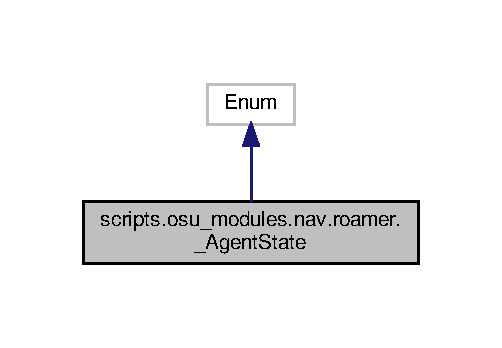
\includegraphics[width=241pt]{dc/dc3/classscripts_1_1osu__modules_1_1nav_1_1roamer_1_1__AgentState__inherit__graph}
\end{center}
\end{figure}


Collaboration diagram for scripts.\+osu\+\_\+modules.\+nav.\+roamer.\+\_\+\+Agent\+State\+:\nopagebreak
\begin{figure}[H]
\begin{center}
\leavevmode
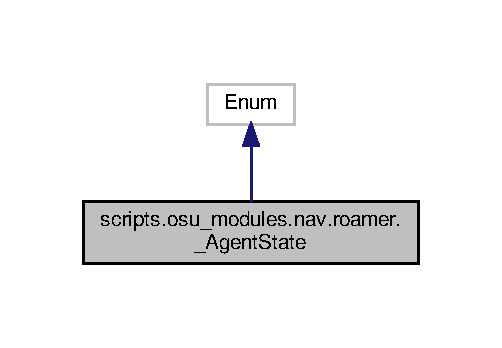
\includegraphics[width=241pt]{d6/d0f/classscripts_1_1osu__modules_1_1nav_1_1roamer_1_1__AgentState__coll__graph}
\end{center}
\end{figure}
\subsection*{Static Public Attributes}
\begin{DoxyCompactItemize}
\item 
\mbox{\Hypertarget{classscripts_1_1osu__modules_1_1nav_1_1roamer_1_1__AgentState_ad4d7451ce9be373b784c07eb7dbd4c21}\label{classscripts_1_1osu__modules_1_1nav_1_1roamer_1_1__AgentState_ad4d7451ce9be373b784c07eb7dbd4c21}} 
int {\bfseries N\+A\+V\+I\+G\+A\+T\+I\+NG} = 1
\item 
\mbox{\Hypertarget{classscripts_1_1osu__modules_1_1nav_1_1roamer_1_1__AgentState_a5defe35453ddb81d1eb2ffaab7339c1e}\label{classscripts_1_1osu__modules_1_1nav_1_1roamer_1_1__AgentState_a5defe35453ddb81d1eb2ffaab7339c1e}} 
int {\bfseries B\+L\+O\+C\+K\+E\+D\+\_\+\+B\+Y\+\_\+\+V\+E\+H\+I\+C\+LE} = 2
\item 
\mbox{\Hypertarget{classscripts_1_1osu__modules_1_1nav_1_1roamer_1_1__AgentState_ae292db8d750efc3cfb3b1071b07aa81a}\label{classscripts_1_1osu__modules_1_1nav_1_1roamer_1_1__AgentState_ae292db8d750efc3cfb3b1071b07aa81a}} 
int {\bfseries B\+L\+O\+C\+K\+E\+D\+\_\+\+R\+E\+D\+\_\+\+L\+I\+G\+HT} = 3
\end{DoxyCompactItemize}


\subsection{Detailed Description}
\begin{DoxyVerb}AGENT_STATE represents the possible states of a roaming agent
\end{DoxyVerb}
 

Definition at line 13 of file roamer.\+py.



The documentation for this class was generated from the following file\+:\begin{DoxyCompactItemize}
\item 
osu\+\_\+modules/nav/roamer.\+py\end{DoxyCompactItemize}

\hypertarget{classscripts_1_1agents_1_1navigation_1_1agent_1_1Agent}{}\section{scripts.\+agents.\+navigation.\+agent.\+Agent Class Reference}
\label{classscripts_1_1agents_1_1navigation_1_1agent_1_1Agent}\index{scripts.\+agents.\+navigation.\+agent.\+Agent@{scripts.\+agents.\+navigation.\+agent.\+Agent}}


Inheritance diagram for scripts.\+agents.\+navigation.\+agent.\+Agent\+:\nopagebreak
\begin{figure}[H]
\begin{center}
\leavevmode
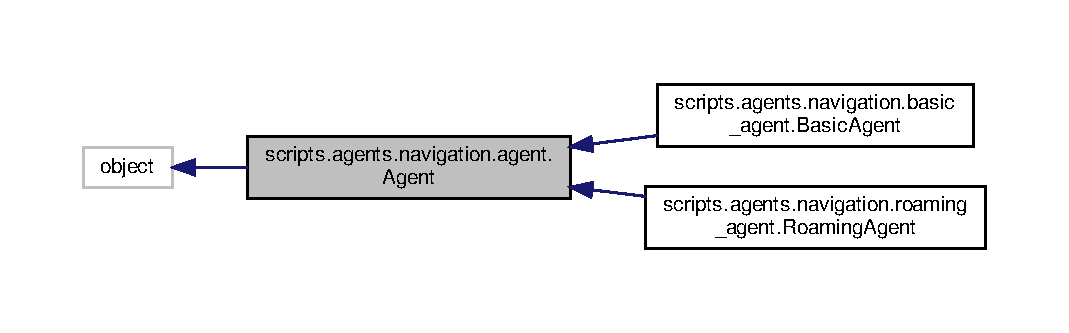
\includegraphics[width=350pt]{d5/d7e/classscripts_1_1agents_1_1navigation_1_1agent_1_1Agent__inherit__graph}
\end{center}
\end{figure}


Collaboration diagram for scripts.\+agents.\+navigation.\+agent.\+Agent\+:\nopagebreak
\begin{figure}[H]
\begin{center}
\leavevmode
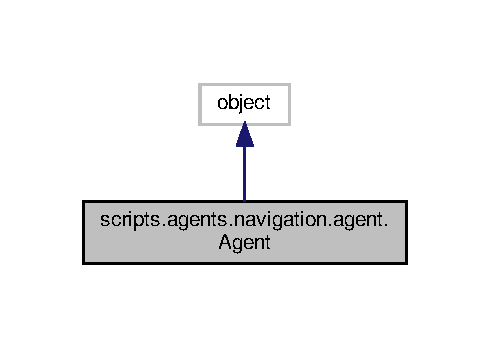
\includegraphics[width=235pt]{de/d72/classscripts_1_1agents_1_1navigation_1_1agent_1_1Agent__coll__graph}
\end{center}
\end{figure}
\subsection*{Public Member Functions}
\begin{DoxyCompactItemize}
\item 
def \hyperlink{classscripts_1_1agents_1_1navigation_1_1agent_1_1Agent_a0e2995e9cfb9a78b724338a26f565c13}{\+\_\+\+\_\+init\+\_\+\+\_\+} (self, vehicle)
\item 
def \hyperlink{classscripts_1_1agents_1_1navigation_1_1agent_1_1Agent_a0271d9ffb0c84bae593bce700a9cf5bc}{run\+\_\+step} (self, debug=False)
\item 
def \hyperlink{classscripts_1_1agents_1_1navigation_1_1agent_1_1Agent_a6c3c4d0e421923e9c4f1bbd478c1f9ea}{emergency\+\_\+stop} (self)
\end{DoxyCompactItemize}


\subsection{Detailed Description}
\begin{DoxyVerb}Base class to define agents in CARLA
\end{DoxyVerb}
 

Definition at line 28 of file agent.\+py.



\subsection{Constructor \& Destructor Documentation}
\mbox{\Hypertarget{classscripts_1_1agents_1_1navigation_1_1agent_1_1Agent_a0e2995e9cfb9a78b724338a26f565c13}\label{classscripts_1_1agents_1_1navigation_1_1agent_1_1Agent_a0e2995e9cfb9a78b724338a26f565c13}} 
\index{scripts\+::agents\+::navigation\+::agent\+::\+Agent@{scripts\+::agents\+::navigation\+::agent\+::\+Agent}!\+\_\+\+\_\+init\+\_\+\+\_\+@{\+\_\+\+\_\+init\+\_\+\+\_\+}}
\index{\+\_\+\+\_\+init\+\_\+\+\_\+@{\+\_\+\+\_\+init\+\_\+\+\_\+}!scripts\+::agents\+::navigation\+::agent\+::\+Agent@{scripts\+::agents\+::navigation\+::agent\+::\+Agent}}
\subsubsection{\texorpdfstring{\+\_\+\+\_\+init\+\_\+\+\_\+()}{\_\_init\_\_()}}
{\footnotesize\ttfamily def scripts.\+agents.\+navigation.\+agent.\+Agent.\+\_\+\+\_\+init\+\_\+\+\_\+ (\begin{DoxyParamCaption}\item[{}]{self,  }\item[{}]{vehicle }\end{DoxyParamCaption})}

\begin{DoxyVerb}:param vehicle: actor to apply to local planner logic onto
\end{DoxyVerb}
 

Definition at line 33 of file agent.\+py.



\subsection{Member Function Documentation}
\mbox{\Hypertarget{classscripts_1_1agents_1_1navigation_1_1agent_1_1Agent_a6c3c4d0e421923e9c4f1bbd478c1f9ea}\label{classscripts_1_1agents_1_1navigation_1_1agent_1_1Agent_a6c3c4d0e421923e9c4f1bbd478c1f9ea}} 
\index{scripts\+::agents\+::navigation\+::agent\+::\+Agent@{scripts\+::agents\+::navigation\+::agent\+::\+Agent}!emergency\+\_\+stop@{emergency\+\_\+stop}}
\index{emergency\+\_\+stop@{emergency\+\_\+stop}!scripts\+::agents\+::navigation\+::agent\+::\+Agent@{scripts\+::agents\+::navigation\+::agent\+::\+Agent}}
\subsubsection{\texorpdfstring{emergency\+\_\+stop()}{emergency\_stop()}}
{\footnotesize\ttfamily def scripts.\+agents.\+navigation.\+agent.\+Agent.\+emergency\+\_\+stop (\begin{DoxyParamCaption}\item[{}]{self }\end{DoxyParamCaption})}

\begin{DoxyVerb}Send an emergency stop command to the vehicle
:return:
\end{DoxyVerb}
 

Definition at line 195 of file agent.\+py.

\mbox{\Hypertarget{classscripts_1_1agents_1_1navigation_1_1agent_1_1Agent_a0271d9ffb0c84bae593bce700a9cf5bc}\label{classscripts_1_1agents_1_1navigation_1_1agent_1_1Agent_a0271d9ffb0c84bae593bce700a9cf5bc}} 
\index{scripts\+::agents\+::navigation\+::agent\+::\+Agent@{scripts\+::agents\+::navigation\+::agent\+::\+Agent}!run\+\_\+step@{run\+\_\+step}}
\index{run\+\_\+step@{run\+\_\+step}!scripts\+::agents\+::navigation\+::agent\+::\+Agent@{scripts\+::agents\+::navigation\+::agent\+::\+Agent}}
\subsubsection{\texorpdfstring{run\+\_\+step()}{run\_step()}}
{\footnotesize\ttfamily def scripts.\+agents.\+navigation.\+agent.\+Agent.\+run\+\_\+step (\begin{DoxyParamCaption}\item[{}]{self,  }\item[{}]{debug = {\ttfamily False} }\end{DoxyParamCaption})}

\begin{DoxyVerb}Execute one step of navigation.
:return: control
\end{DoxyVerb}
 

Definition at line 45 of file agent.\+py.



The documentation for this class was generated from the following file\+:\begin{DoxyCompactItemize}
\item 
agents/navigation/agent.\+py\end{DoxyCompactItemize}

\hypertarget{classscripts_1_1agents_1_1navigation_1_1agent_1_1AgentState}{}\section{scripts.\+agents.\+navigation.\+agent.\+Agent\+State Class Reference}
\label{classscripts_1_1agents_1_1navigation_1_1agent_1_1AgentState}\index{scripts.\+agents.\+navigation.\+agent.\+Agent\+State@{scripts.\+agents.\+navigation.\+agent.\+Agent\+State}}


Inheritance diagram for scripts.\+agents.\+navigation.\+agent.\+Agent\+State\+:\nopagebreak
\begin{figure}[H]
\begin{center}
\leavevmode
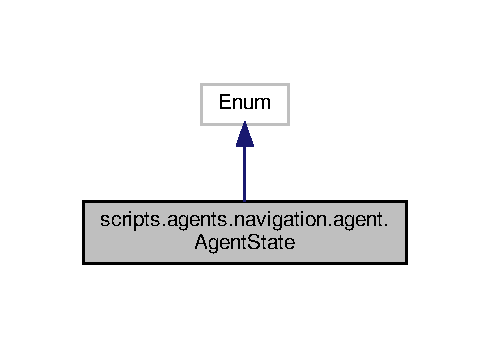
\includegraphics[width=235pt]{d4/dd3/classscripts_1_1agents_1_1navigation_1_1agent_1_1AgentState__inherit__graph}
\end{center}
\end{figure}


Collaboration diagram for scripts.\+agents.\+navigation.\+agent.\+Agent\+State\+:\nopagebreak
\begin{figure}[H]
\begin{center}
\leavevmode
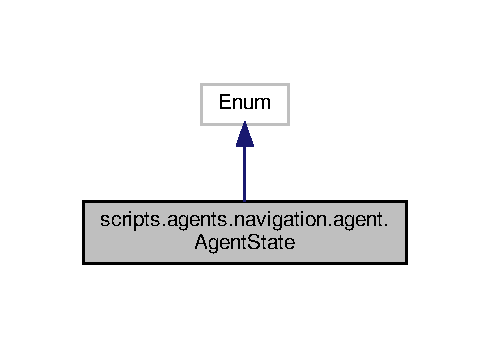
\includegraphics[width=235pt]{da/d74/classscripts_1_1agents_1_1navigation_1_1agent_1_1AgentState__coll__graph}
\end{center}
\end{figure}
\subsection*{Static Public Attributes}
\begin{DoxyCompactItemize}
\item 
\mbox{\Hypertarget{classscripts_1_1agents_1_1navigation_1_1agent_1_1AgentState_a3321c6caf55a1de76918ed9f4dbebb6a}\label{classscripts_1_1agents_1_1navigation_1_1agent_1_1AgentState_a3321c6caf55a1de76918ed9f4dbebb6a}} 
int {\bfseries N\+A\+V\+I\+G\+A\+T\+I\+NG} = 1
\item 
\mbox{\Hypertarget{classscripts_1_1agents_1_1navigation_1_1agent_1_1AgentState_a1f7326a0dca7607a98705a55d56ffd4c}\label{classscripts_1_1agents_1_1navigation_1_1agent_1_1AgentState_a1f7326a0dca7607a98705a55d56ffd4c}} 
int {\bfseries B\+L\+O\+C\+K\+E\+D\+\_\+\+B\+Y\+\_\+\+V\+E\+H\+I\+C\+LE} = 2
\item 
\mbox{\Hypertarget{classscripts_1_1agents_1_1navigation_1_1agent_1_1AgentState_ac2885971cbdb0fc594f7686ac5c49804}\label{classscripts_1_1agents_1_1navigation_1_1agent_1_1AgentState_ac2885971cbdb0fc594f7686ac5c49804}} 
int {\bfseries B\+L\+O\+C\+K\+E\+D\+\_\+\+R\+E\+D\+\_\+\+L\+I\+G\+HT} = 3
\end{DoxyCompactItemize}


\subsection{Detailed Description}
\begin{DoxyVerb}AGENT_STATE represents the possible states of a roaming agent
\end{DoxyVerb}
 

Definition at line 19 of file agent.\+py.



The documentation for this class was generated from the following file\+:\begin{DoxyCompactItemize}
\item 
agents/navigation/agent.\+py\end{DoxyCompactItemize}

\hypertarget{classtest__AV__control_1_1AV}{}\section{test\+\_\+\+A\+V\+\_\+control.\+AV Class Reference}
\label{classtest__AV__control_1_1AV}\index{test\+\_\+\+A\+V\+\_\+control.\+AV@{test\+\_\+\+A\+V\+\_\+control.\+AV}}


\hyperlink{classtest__AV__control_1_1AV}{AV} class.  




Inheritance diagram for test\+\_\+\+A\+V\+\_\+control.\+AV\+:\nopagebreak
\begin{figure}[H]
\begin{center}
\leavevmode
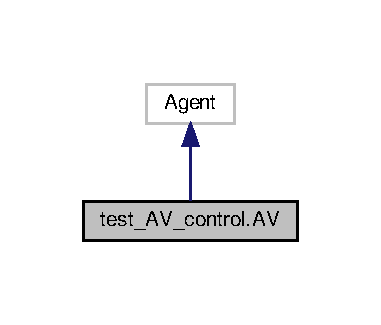
\includegraphics[width=183pt]{d5/d53/classtest__AV__control_1_1AV__inherit__graph}
\end{center}
\end{figure}


Collaboration diagram for test\+\_\+\+A\+V\+\_\+control.\+AV\+:\nopagebreak
\begin{figure}[H]
\begin{center}
\leavevmode
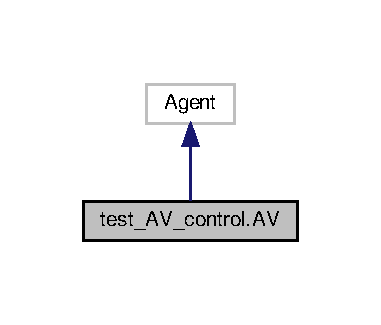
\includegraphics[width=183pt]{da/d5b/classtest__AV__control_1_1AV__coll__graph}
\end{center}
\end{figure}
\subsection*{Public Member Functions}
\begin{DoxyCompactItemize}
\item 
\mbox{\Hypertarget{classtest__AV__control_1_1AV_aa16b44e2795d96ee898307a467ebb22a}\label{classtest__AV__control_1_1AV_aa16b44e2795d96ee898307a467ebb22a}} 
def {\bfseries \+\_\+\+\_\+init\+\_\+\+\_\+} (self, vehicle)
\item 
\mbox{\Hypertarget{classtest__AV__control_1_1AV_ab638809ebc044a4d8dbdf703d5831479}\label{classtest__AV__control_1_1AV_ab638809ebc044a4d8dbdf703d5831479}} 
def {\bfseries update\+\_\+status} (self, vehicle\+\_\+status)
\end{DoxyCompactItemize}
\subsection*{Public Attributes}
\begin{DoxyCompactItemize}
\item 
\mbox{\Hypertarget{classtest__AV__control_1_1AV_a920ffe826ec8ab67d319ec238561a79a}\label{classtest__AV__control_1_1AV_a920ffe826ec8ab67d319ec238561a79a}} 
{\bfseries vehicle\+\_\+state}
\end{DoxyCompactItemize}


\subsection{Detailed Description}
\hyperlink{classtest__AV__control_1_1AV}{AV} class. 

Definition at line 40 of file test\+\_\+\+A\+V\+\_\+control.\+py.



The documentation for this class was generated from the following file\+:\begin{DoxyCompactItemize}
\item 
osu\+\_\+modules/tests/test\+\_\+\+A\+V\+\_\+control.\+py\end{DoxyCompactItemize}

\hypertarget{classscripts_1_1osu__modules_1_1dynamics_1_1av_1_1AV}{}\section{scripts.\+osu\+\_\+modules.\+dynamics.\+av.\+AV Class Reference}
\label{classscripts_1_1osu__modules_1_1dynamics_1_1av_1_1AV}\index{scripts.\+osu\+\_\+modules.\+dynamics.\+av.\+AV@{scripts.\+osu\+\_\+modules.\+dynamics.\+av.\+AV}}


Inheritance diagram for scripts.\+osu\+\_\+modules.\+dynamics.\+av.\+AV\+:
\nopagebreak
\begin{figure}[H]
\begin{center}
\leavevmode
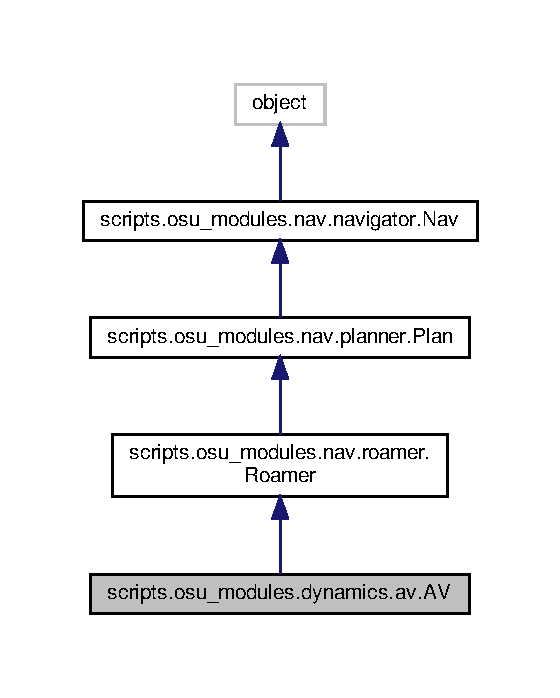
\includegraphics[width=269pt]{d4/d15/classscripts_1_1osu__modules_1_1dynamics_1_1av_1_1AV__inherit__graph}
\end{center}
\end{figure}


Collaboration diagram for scripts.\+osu\+\_\+modules.\+dynamics.\+av.\+AV\+:
\nopagebreak
\begin{figure}[H]
\begin{center}
\leavevmode
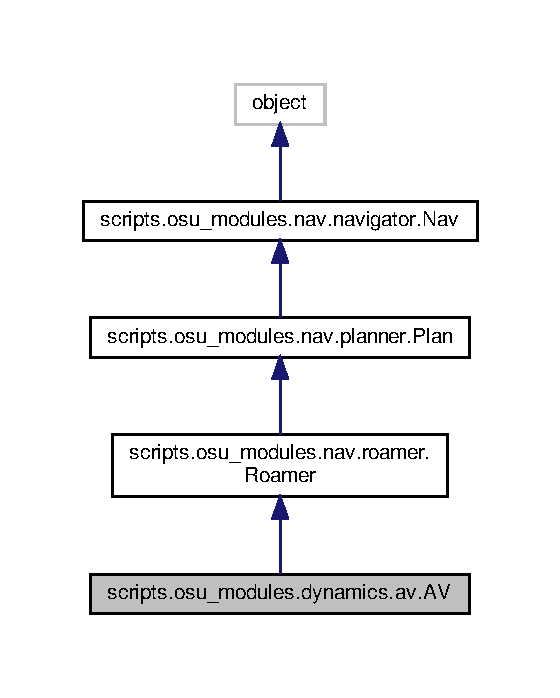
\includegraphics[width=269pt]{d5/db2/classscripts_1_1osu__modules_1_1dynamics_1_1av_1_1AV__coll__graph}
\end{center}
\end{figure}
\subsection*{Public Member Functions}
\begin{DoxyCompactItemize}
\item 
\mbox{\Hypertarget{classscripts_1_1osu__modules_1_1dynamics_1_1av_1_1AV_a89f85341e7a2c217b2e394eb0f9d8816}\label{classscripts_1_1osu__modules_1_1dynamics_1_1av_1_1AV_a89f85341e7a2c217b2e394eb0f9d8816}} 
def {\bfseries \+\_\+\+\_\+init\+\_\+\+\_\+} (self, world, vehicle\+\_\+local)
\end{DoxyCompactItemize}
\subsection*{Public Attributes}
\begin{DoxyCompactItemize}
\item 
\mbox{\Hypertarget{classscripts_1_1osu__modules_1_1dynamics_1_1av_1_1AV_ab12b622df5432d4405ed2cba87cac411}\label{classscripts_1_1osu__modules_1_1dynamics_1_1av_1_1AV_ab12b622df5432d4405ed2cba87cac411}} 
{\bfseries role\+\_\+name}
\item 
\mbox{\Hypertarget{classscripts_1_1osu__modules_1_1dynamics_1_1av_1_1AV_aa1fc87332f3b17fe88d839b09241324d}\label{classscripts_1_1osu__modules_1_1dynamics_1_1av_1_1AV_aa1fc87332f3b17fe88d839b09241324d}} 
{\bfseries control\+\_\+vel\+\_\+subscriber}
\item 
\mbox{\Hypertarget{classscripts_1_1osu__modules_1_1dynamics_1_1av_1_1AV_a6683aab7732c2ef6842fa6a0d8c99d43}\label{classscripts_1_1osu__modules_1_1dynamics_1_1av_1_1AV_a6683aab7732c2ef6842fa6a0d8c99d43}} 
{\bfseries control\+\_\+steering\+\_\+subscriber}
\item 
\mbox{\Hypertarget{classscripts_1_1osu__modules_1_1dynamics_1_1av_1_1AV_a48a7aefaf17b0f77313e5d556f025b93}\label{classscripts_1_1osu__modules_1_1dynamics_1_1av_1_1AV_a48a7aefaf17b0f77313e5d556f025b93}} 
{\bfseries test\+\_\+subscriber}
\item 
\mbox{\Hypertarget{classscripts_1_1osu__modules_1_1dynamics_1_1av_1_1AV_a9ae65cc37983a1b95a68f67b4a670afb}\label{classscripts_1_1osu__modules_1_1dynamics_1_1av_1_1AV_a9ae65cc37983a1b95a68f67b4a670afb}} 
{\bfseries carla\+\_\+set\+\_\+publisher}
\item 
\mbox{\Hypertarget{classscripts_1_1osu__modules_1_1dynamics_1_1av_1_1AV_ac6c2af296c766e6d422f0711bf668bfe}\label{classscripts_1_1osu__modules_1_1dynamics_1_1av_1_1AV_ac6c2af296c766e6d422f0711bf668bfe}} 
{\bfseries carla\+\_\+path\+\_\+publisher}
\item 
\mbox{\Hypertarget{classscripts_1_1osu__modules_1_1dynamics_1_1av_1_1AV_a62a2e2142973b226f4fa69aed60a7598}\label{classscripts_1_1osu__modules_1_1dynamics_1_1av_1_1AV_a62a2e2142973b226f4fa69aed60a7598}} 
{\bfseries carla\+\_\+path\+\_\+publisher\+\_\+act}
\end{DoxyCompactItemize}
\subsection*{Static Public Attributes}
\begin{DoxyCompactItemize}
\item 
\mbox{\Hypertarget{classscripts_1_1osu__modules_1_1dynamics_1_1av_1_1AV_aadd1c0d9afe9e5fbb9bcc4b1b0c24c79}\label{classscripts_1_1osu__modules_1_1dynamics_1_1av_1_1AV_aadd1c0d9afe9e5fbb9bcc4b1b0c24c79}} 
{\bfseries rh} = \hyperlink{classscripts_1_1osu__modules_1_1tools_1_1robotic__helper_1_1RoboticHelper}{Robotic\+Helper}()
\item 
{\bfseries world\+\_\+orientation}
\end{DoxyCompactItemize}


\subsection{Detailed Description}
\begin{DoxyVerb}Autonomous Vehicle class used to operate carla vehicle

    super Roamer determines path
    uses VehicleVelocityControl to operate vehicle
\end{DoxyVerb}
 

Definition at line 27 of file av.\+py.



\subsection{Member Data Documentation}
\mbox{\Hypertarget{classscripts_1_1osu__modules_1_1dynamics_1_1av_1_1AV_a8adc74df27841b930510ddeaefe7e4d2}\label{classscripts_1_1osu__modules_1_1dynamics_1_1av_1_1AV_a8adc74df27841b930510ddeaefe7e4d2}} 
\index{scripts\+::osu\+\_\+modules\+::dynamics\+::av\+::\+AV@{scripts\+::osu\+\_\+modules\+::dynamics\+::av\+::\+AV}!world\+\_\+orientation@{world\+\_\+orientation}}
\index{world\+\_\+orientation@{world\+\_\+orientation}!scripts\+::osu\+\_\+modules\+::dynamics\+::av\+::\+AV@{scripts\+::osu\+\_\+modules\+::dynamics\+::av\+::\+AV}}
\subsubsection{\texorpdfstring{world\+\_\+orientation}{world\_orientation}}
{\footnotesize\ttfamily scripts.\+osu\+\_\+modules.\+dynamics.\+av.\+A\+V.\+world\+\_\+orientation\hspace{0.3cm}{\ttfamily [static]}}

{\bfseries Initial value\+:}
\begin{DoxyCode}
=  np.array([[1, 0, 0],
                                  [0, 1, 0],
                                  [0, 0, -1]])
\end{DoxyCode}


Definition at line 39 of file av.\+py.



The documentation for this class was generated from the following file\+:\begin{DoxyCompactItemize}
\item 
osu\+\_\+modules/dynamics/av.\+py\end{DoxyCompactItemize}

\hypertarget{classscripts_1_1agents_1_1navigation_1_1basic__agent_1_1BasicAgent}{}\section{scripts.\+agents.\+navigation.\+basic\+\_\+agent.\+Basic\+Agent Class Reference}
\label{classscripts_1_1agents_1_1navigation_1_1basic__agent_1_1BasicAgent}\index{scripts.\+agents.\+navigation.\+basic\+\_\+agent.\+Basic\+Agent@{scripts.\+agents.\+navigation.\+basic\+\_\+agent.\+Basic\+Agent}}


Inheritance diagram for scripts.\+agents.\+navigation.\+basic\+\_\+agent.\+Basic\+Agent\+:\nopagebreak
\begin{figure}[H]
\begin{center}
\leavevmode
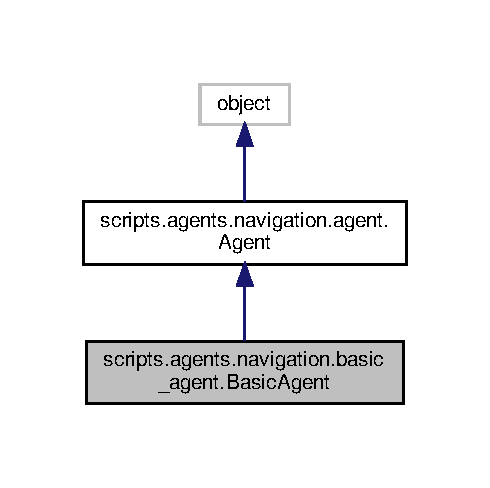
\includegraphics[width=235pt]{d7/d3d/classscripts_1_1agents_1_1navigation_1_1basic__agent_1_1BasicAgent__inherit__graph}
\end{center}
\end{figure}


Collaboration diagram for scripts.\+agents.\+navigation.\+basic\+\_\+agent.\+Basic\+Agent\+:\nopagebreak
\begin{figure}[H]
\begin{center}
\leavevmode
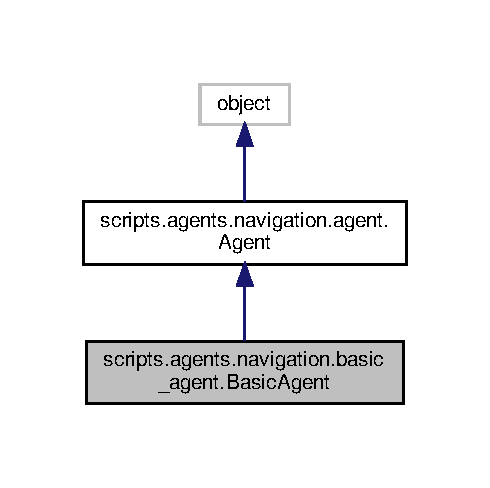
\includegraphics[width=235pt]{dd/ddc/classscripts_1_1agents_1_1navigation_1_1basic__agent_1_1BasicAgent__coll__graph}
\end{center}
\end{figure}
\subsection*{Public Member Functions}
\begin{DoxyCompactItemize}
\item 
def \hyperlink{classscripts_1_1agents_1_1navigation_1_1basic__agent_1_1BasicAgent_a69580567044bfe09eba8da5bebd89beb}{\+\_\+\+\_\+init\+\_\+\+\_\+} (self, vehicle, target\+\_\+speed=20)
\item 
def \hyperlink{classscripts_1_1agents_1_1navigation_1_1basic__agent_1_1BasicAgent_acccc65ae1b4c49557f59b83eb9bc1502}{set\+\_\+destination} (self, location)
\item 
def \hyperlink{classscripts_1_1agents_1_1navigation_1_1basic__agent_1_1BasicAgent_aa6ae836338e7fe24be266108cfe99894}{run\+\_\+step} (self, debug=False)
\end{DoxyCompactItemize}


\subsection{Detailed Description}
\begin{DoxyVerb}BasicAgent implements a basic agent that navigates scenes to reach a given
target destination. This agent respects traffic lights and other vehicles.
\end{DoxyVerb}
 

Definition at line 20 of file basic\+\_\+agent.\+py.



\subsection{Constructor \& Destructor Documentation}
\mbox{\Hypertarget{classscripts_1_1agents_1_1navigation_1_1basic__agent_1_1BasicAgent_a69580567044bfe09eba8da5bebd89beb}\label{classscripts_1_1agents_1_1navigation_1_1basic__agent_1_1BasicAgent_a69580567044bfe09eba8da5bebd89beb}} 
\index{scripts\+::agents\+::navigation\+::basic\+\_\+agent\+::\+Basic\+Agent@{scripts\+::agents\+::navigation\+::basic\+\_\+agent\+::\+Basic\+Agent}!\+\_\+\+\_\+init\+\_\+\+\_\+@{\+\_\+\+\_\+init\+\_\+\+\_\+}}
\index{\+\_\+\+\_\+init\+\_\+\+\_\+@{\+\_\+\+\_\+init\+\_\+\+\_\+}!scripts\+::agents\+::navigation\+::basic\+\_\+agent\+::\+Basic\+Agent@{scripts\+::agents\+::navigation\+::basic\+\_\+agent\+::\+Basic\+Agent}}
\subsubsection{\texorpdfstring{\+\_\+\+\_\+init\+\_\+\+\_\+()}{\_\_init\_\_()}}
{\footnotesize\ttfamily def scripts.\+agents.\+navigation.\+basic\+\_\+agent.\+Basic\+Agent.\+\_\+\+\_\+init\+\_\+\+\_\+ (\begin{DoxyParamCaption}\item[{}]{self,  }\item[{}]{vehicle,  }\item[{}]{target\+\_\+speed = {\ttfamily 20} }\end{DoxyParamCaption})}

\begin{DoxyVerb}:param vehicle: actor to apply to local planner logic onto
\end{DoxyVerb}
 

Definition at line 26 of file basic\+\_\+agent.\+py.



\subsection{Member Function Documentation}
\mbox{\Hypertarget{classscripts_1_1agents_1_1navigation_1_1basic__agent_1_1BasicAgent_aa6ae836338e7fe24be266108cfe99894}\label{classscripts_1_1agents_1_1navigation_1_1basic__agent_1_1BasicAgent_aa6ae836338e7fe24be266108cfe99894}} 
\index{scripts\+::agents\+::navigation\+::basic\+\_\+agent\+::\+Basic\+Agent@{scripts\+::agents\+::navigation\+::basic\+\_\+agent\+::\+Basic\+Agent}!run\+\_\+step@{run\+\_\+step}}
\index{run\+\_\+step@{run\+\_\+step}!scripts\+::agents\+::navigation\+::basic\+\_\+agent\+::\+Basic\+Agent@{scripts\+::agents\+::navigation\+::basic\+\_\+agent\+::\+Basic\+Agent}}
\subsubsection{\texorpdfstring{run\+\_\+step()}{run\_step()}}
{\footnotesize\ttfamily def scripts.\+agents.\+navigation.\+basic\+\_\+agent.\+Basic\+Agent.\+run\+\_\+step (\begin{DoxyParamCaption}\item[{}]{self,  }\item[{}]{debug = {\ttfamily False} }\end{DoxyParamCaption})}

\begin{DoxyVerb}Execute one step of navigation.
:return: carla.VehicleControl
\end{DoxyVerb}
 

Definition at line 84 of file basic\+\_\+agent.\+py.

\mbox{\Hypertarget{classscripts_1_1agents_1_1navigation_1_1basic__agent_1_1BasicAgent_acccc65ae1b4c49557f59b83eb9bc1502}\label{classscripts_1_1agents_1_1navigation_1_1basic__agent_1_1BasicAgent_acccc65ae1b4c49557f59b83eb9bc1502}} 
\index{scripts\+::agents\+::navigation\+::basic\+\_\+agent\+::\+Basic\+Agent@{scripts\+::agents\+::navigation\+::basic\+\_\+agent\+::\+Basic\+Agent}!set\+\_\+destination@{set\+\_\+destination}}
\index{set\+\_\+destination@{set\+\_\+destination}!scripts\+::agents\+::navigation\+::basic\+\_\+agent\+::\+Basic\+Agent@{scripts\+::agents\+::navigation\+::basic\+\_\+agent\+::\+Basic\+Agent}}
\subsubsection{\texorpdfstring{set\+\_\+destination()}{set\_destination()}}
{\footnotesize\ttfamily def scripts.\+agents.\+navigation.\+basic\+\_\+agent.\+Basic\+Agent.\+set\+\_\+destination (\begin{DoxyParamCaption}\item[{}]{self,  }\item[{}]{location }\end{DoxyParamCaption})}

\begin{DoxyVerb}This method creates a list of waypoints from agent's position to destination location
based on the route returned by the global router
\end{DoxyVerb}
 

Definition at line 49 of file basic\+\_\+agent.\+py.



The documentation for this class was generated from the following file\+:\begin{DoxyCompactItemize}
\item 
agents/navigation/basic\+\_\+agent.\+py\end{DoxyCompactItemize}

\hypertarget{classscripts_1_1agents_1_1navigation_1_1global__route__planner_1_1GlobalRoutePlanner}{}\section{scripts.\+agents.\+navigation.\+global\+\_\+route\+\_\+planner.\+Global\+Route\+Planner Class Reference}
\label{classscripts_1_1agents_1_1navigation_1_1global__route__planner_1_1GlobalRoutePlanner}\index{scripts.\+agents.\+navigation.\+global\+\_\+route\+\_\+planner.\+Global\+Route\+Planner@{scripts.\+agents.\+navigation.\+global\+\_\+route\+\_\+planner.\+Global\+Route\+Planner}}


Inheritance diagram for scripts.\+agents.\+navigation.\+global\+\_\+route\+\_\+planner.\+Global\+Route\+Planner\+:\nopagebreak
\begin{figure}[H]
\begin{center}
\leavevmode
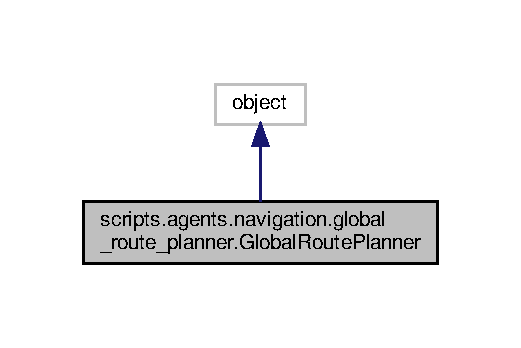
\includegraphics[width=250pt]{d8/d27/classscripts_1_1agents_1_1navigation_1_1global__route__planner_1_1GlobalRoutePlanner__inherit__graph}
\end{center}
\end{figure}


Collaboration diagram for scripts.\+agents.\+navigation.\+global\+\_\+route\+\_\+planner.\+Global\+Route\+Planner\+:\nopagebreak
\begin{figure}[H]
\begin{center}
\leavevmode
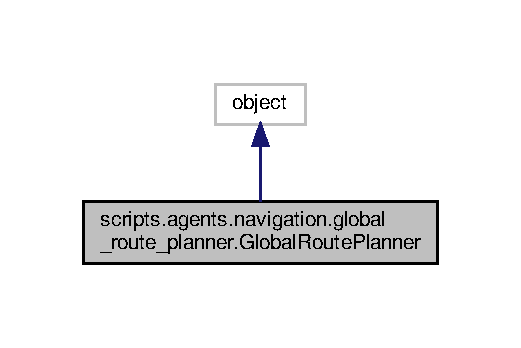
\includegraphics[width=250pt]{db/db5/classscripts_1_1agents_1_1navigation_1_1global__route__planner_1_1GlobalRoutePlanner__coll__graph}
\end{center}
\end{figure}
\subsection*{Public Member Functions}
\begin{DoxyCompactItemize}
\item 
def \hyperlink{classscripts_1_1agents_1_1navigation_1_1global__route__planner_1_1GlobalRoutePlanner_a22be77eb07fc0532b5cb0c03e365cee0}{\+\_\+\+\_\+init\+\_\+\+\_\+} (self, dao)
\item 
def \hyperlink{classscripts_1_1agents_1_1navigation_1_1global__route__planner_1_1GlobalRoutePlanner_a1d5a29b9a1796bc9e1eaab60bc82f0f3}{setup} (self)
\item 
def \hyperlink{classscripts_1_1agents_1_1navigation_1_1global__route__planner_1_1GlobalRoutePlanner_a185c36e8f776da7fe7825e80a09267d9}{abstract\+\_\+route\+\_\+plan} (self, origin, destination)
\item 
def \hyperlink{classscripts_1_1agents_1_1navigation_1_1global__route__planner_1_1GlobalRoutePlanner_a0e1e3890e3adafbbb3acdb213c3077ff}{trace\+\_\+route} (self, origin, destination)
\end{DoxyCompactItemize}


\subsection{Detailed Description}
\begin{DoxyVerb}This class provides a very high level route plan.
Instantiate the class by passing a reference to
A GlobalRoutePlannerDAO object.
\end{DoxyVerb}
 

Definition at line 18 of file global\+\_\+route\+\_\+planner.\+py.



\subsection{Constructor \& Destructor Documentation}
\mbox{\Hypertarget{classscripts_1_1agents_1_1navigation_1_1global__route__planner_1_1GlobalRoutePlanner_a22be77eb07fc0532b5cb0c03e365cee0}\label{classscripts_1_1agents_1_1navigation_1_1global__route__planner_1_1GlobalRoutePlanner_a22be77eb07fc0532b5cb0c03e365cee0}} 
\index{scripts\+::agents\+::navigation\+::global\+\_\+route\+\_\+planner\+::\+Global\+Route\+Planner@{scripts\+::agents\+::navigation\+::global\+\_\+route\+\_\+planner\+::\+Global\+Route\+Planner}!\+\_\+\+\_\+init\+\_\+\+\_\+@{\+\_\+\+\_\+init\+\_\+\+\_\+}}
\index{\+\_\+\+\_\+init\+\_\+\+\_\+@{\+\_\+\+\_\+init\+\_\+\+\_\+}!scripts\+::agents\+::navigation\+::global\+\_\+route\+\_\+planner\+::\+Global\+Route\+Planner@{scripts\+::agents\+::navigation\+::global\+\_\+route\+\_\+planner\+::\+Global\+Route\+Planner}}
\subsubsection{\texorpdfstring{\+\_\+\+\_\+init\+\_\+\+\_\+()}{\_\_init\_\_()}}
{\footnotesize\ttfamily def scripts.\+agents.\+navigation.\+global\+\_\+route\+\_\+planner.\+Global\+Route\+Planner.\+\_\+\+\_\+init\+\_\+\+\_\+ (\begin{DoxyParamCaption}\item[{}]{self,  }\item[{}]{dao }\end{DoxyParamCaption})}

\begin{DoxyVerb}Constructor
\end{DoxyVerb}
 

Definition at line 25 of file global\+\_\+route\+\_\+planner.\+py.



\subsection{Member Function Documentation}
\mbox{\Hypertarget{classscripts_1_1agents_1_1navigation_1_1global__route__planner_1_1GlobalRoutePlanner_a185c36e8f776da7fe7825e80a09267d9}\label{classscripts_1_1agents_1_1navigation_1_1global__route__planner_1_1GlobalRoutePlanner_a185c36e8f776da7fe7825e80a09267d9}} 
\index{scripts\+::agents\+::navigation\+::global\+\_\+route\+\_\+planner\+::\+Global\+Route\+Planner@{scripts\+::agents\+::navigation\+::global\+\_\+route\+\_\+planner\+::\+Global\+Route\+Planner}!abstract\+\_\+route\+\_\+plan@{abstract\+\_\+route\+\_\+plan}}
\index{abstract\+\_\+route\+\_\+plan@{abstract\+\_\+route\+\_\+plan}!scripts\+::agents\+::navigation\+::global\+\_\+route\+\_\+planner\+::\+Global\+Route\+Planner@{scripts\+::agents\+::navigation\+::global\+\_\+route\+\_\+planner\+::\+Global\+Route\+Planner}}
\subsubsection{\texorpdfstring{abstract\+\_\+route\+\_\+plan()}{abstract\_route\_plan()}}
{\footnotesize\ttfamily def scripts.\+agents.\+navigation.\+global\+\_\+route\+\_\+planner.\+Global\+Route\+Planner.\+abstract\+\_\+route\+\_\+plan (\begin{DoxyParamCaption}\item[{}]{self,  }\item[{}]{origin,  }\item[{}]{destination }\end{DoxyParamCaption})}

\begin{DoxyVerb}The following function generates the route plan based on
origin      : carla.Location object of the route's start position
destination : carla.Location object of the route's end position
return      : list of turn by turn navigation decisions as
agents.navigation.local_planner.RoadOption elements
Possible values are STRAIGHT, LEFT, RIGHT, LANEFOLLOW, VOID
CHANGELANELEFT, CHANGELANERIGHT
\end{DoxyVerb}
 

Definition at line 228 of file global\+\_\+route\+\_\+planner.\+py.

\mbox{\Hypertarget{classscripts_1_1agents_1_1navigation_1_1global__route__planner_1_1GlobalRoutePlanner_a1d5a29b9a1796bc9e1eaab60bc82f0f3}\label{classscripts_1_1agents_1_1navigation_1_1global__route__planner_1_1GlobalRoutePlanner_a1d5a29b9a1796bc9e1eaab60bc82f0f3}} 
\index{scripts\+::agents\+::navigation\+::global\+\_\+route\+\_\+planner\+::\+Global\+Route\+Planner@{scripts\+::agents\+::navigation\+::global\+\_\+route\+\_\+planner\+::\+Global\+Route\+Planner}!setup@{setup}}
\index{setup@{setup}!scripts\+::agents\+::navigation\+::global\+\_\+route\+\_\+planner\+::\+Global\+Route\+Planner@{scripts\+::agents\+::navigation\+::global\+\_\+route\+\_\+planner\+::\+Global\+Route\+Planner}}
\subsubsection{\texorpdfstring{setup()}{setup()}}
{\footnotesize\ttfamily def scripts.\+agents.\+navigation.\+global\+\_\+route\+\_\+planner.\+Global\+Route\+Planner.\+setup (\begin{DoxyParamCaption}\item[{}]{self }\end{DoxyParamCaption})}

\begin{DoxyVerb}Performs initial server data lookup for detailed topology
and builds graph representation of the world map.
\end{DoxyVerb}
 

Definition at line 35 of file global\+\_\+route\+\_\+planner.\+py.

\mbox{\Hypertarget{classscripts_1_1agents_1_1navigation_1_1global__route__planner_1_1GlobalRoutePlanner_a0e1e3890e3adafbbb3acdb213c3077ff}\label{classscripts_1_1agents_1_1navigation_1_1global__route__planner_1_1GlobalRoutePlanner_a0e1e3890e3adafbbb3acdb213c3077ff}} 
\index{scripts\+::agents\+::navigation\+::global\+\_\+route\+\_\+planner\+::\+Global\+Route\+Planner@{scripts\+::agents\+::navigation\+::global\+\_\+route\+\_\+planner\+::\+Global\+Route\+Planner}!trace\+\_\+route@{trace\+\_\+route}}
\index{trace\+\_\+route@{trace\+\_\+route}!scripts\+::agents\+::navigation\+::global\+\_\+route\+\_\+planner\+::\+Global\+Route\+Planner@{scripts\+::agents\+::navigation\+::global\+\_\+route\+\_\+planner\+::\+Global\+Route\+Planner}}
\subsubsection{\texorpdfstring{trace\+\_\+route()}{trace\_route()}}
{\footnotesize\ttfamily def scripts.\+agents.\+navigation.\+global\+\_\+route\+\_\+planner.\+Global\+Route\+Planner.\+trace\+\_\+route (\begin{DoxyParamCaption}\item[{}]{self,  }\item[{}]{origin,  }\item[{}]{destination }\end{DoxyParamCaption})}

\begin{DoxyVerb}This method returns list of (carla.Waypoint, RoadOption) from origin to destination
\end{DoxyVerb}
 

Definition at line 260 of file global\+\_\+route\+\_\+planner.\+py.



The documentation for this class was generated from the following file\+:\begin{DoxyCompactItemize}
\item 
agents/navigation/global\+\_\+route\+\_\+planner.\+py\end{DoxyCompactItemize}

\hypertarget{classscripts_1_1agents_1_1navigation_1_1global__route__planner__dao_1_1GlobalRoutePlannerDAO}{}\section{scripts.\+agents.\+navigation.\+global\+\_\+route\+\_\+planner\+\_\+dao.\+Global\+Route\+Planner\+D\+AO Class Reference}
\label{classscripts_1_1agents_1_1navigation_1_1global__route__planner__dao_1_1GlobalRoutePlannerDAO}\index{scripts.\+agents.\+navigation.\+global\+\_\+route\+\_\+planner\+\_\+dao.\+Global\+Route\+Planner\+D\+AO@{scripts.\+agents.\+navigation.\+global\+\_\+route\+\_\+planner\+\_\+dao.\+Global\+Route\+Planner\+D\+AO}}


Inheritance diagram for scripts.\+agents.\+navigation.\+global\+\_\+route\+\_\+planner\+\_\+dao.\+Global\+Route\+Planner\+D\+AO\+:
\nopagebreak
\begin{figure}[H]
\begin{center}
\leavevmode
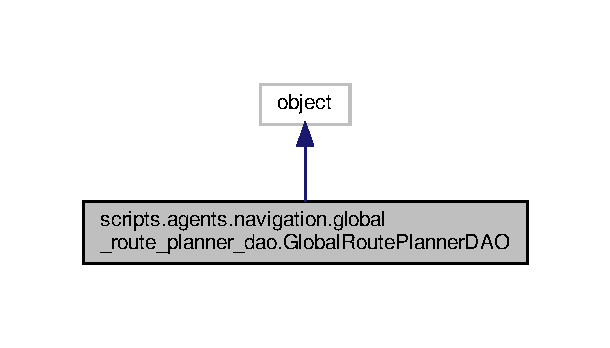
\includegraphics[width=293pt]{d1/dee/classscripts_1_1agents_1_1navigation_1_1global__route__planner__dao_1_1GlobalRoutePlannerDAO__inherit__graph}
\end{center}
\end{figure}


Collaboration diagram for scripts.\+agents.\+navigation.\+global\+\_\+route\+\_\+planner\+\_\+dao.\+Global\+Route\+Planner\+D\+AO\+:
\nopagebreak
\begin{figure}[H]
\begin{center}
\leavevmode
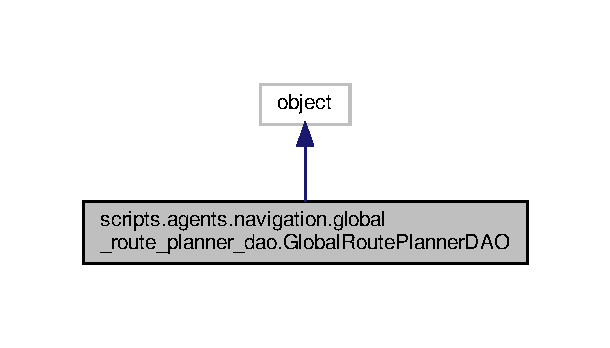
\includegraphics[width=293pt]{db/d72/classscripts_1_1agents_1_1navigation_1_1global__route__planner__dao_1_1GlobalRoutePlannerDAO__coll__graph}
\end{center}
\end{figure}
\subsection*{Public Member Functions}
\begin{DoxyCompactItemize}
\item 
def \hyperlink{classscripts_1_1agents_1_1navigation_1_1global__route__planner__dao_1_1GlobalRoutePlannerDAO_aa6998a36f5e40b3ac35e11f526b910cb}{\+\_\+\+\_\+init\+\_\+\+\_\+} (self, wmap, sampling\+\_\+resolution=1)
\item 
def \hyperlink{classscripts_1_1agents_1_1navigation_1_1global__route__planner__dao_1_1GlobalRoutePlannerDAO_adc57ea46ad2f68901f15e8fb11d097e5}{get\+\_\+topology} (self)
\item 
def \hyperlink{classscripts_1_1agents_1_1navigation_1_1global__route__planner__dao_1_1GlobalRoutePlannerDAO_a30b1db1681843781913b551ea1bf0551}{get\+\_\+waypoint} (self, location)
\item 
def \hyperlink{classscripts_1_1agents_1_1navigation_1_1global__route__planner__dao_1_1GlobalRoutePlannerDAO_a40ee35519bc601af9469dcf0b5fe57f4}{get\+\_\+resolution} (self)
\end{DoxyCompactItemize}


\subsection{Detailed Description}
\begin{DoxyVerb}This class is the data access layer for fetching data
from the carla server instance for GlobalRoutePlanner
\end{DoxyVerb}
 

Definition at line 11 of file global\+\_\+route\+\_\+planner\+\_\+dao.\+py.



\subsection{Constructor \& Destructor Documentation}
\mbox{\Hypertarget{classscripts_1_1agents_1_1navigation_1_1global__route__planner__dao_1_1GlobalRoutePlannerDAO_aa6998a36f5e40b3ac35e11f526b910cb}\label{classscripts_1_1agents_1_1navigation_1_1global__route__planner__dao_1_1GlobalRoutePlannerDAO_aa6998a36f5e40b3ac35e11f526b910cb}} 
\index{scripts\+::agents\+::navigation\+::global\+\_\+route\+\_\+planner\+\_\+dao\+::\+Global\+Route\+Planner\+D\+AO@{scripts\+::agents\+::navigation\+::global\+\_\+route\+\_\+planner\+\_\+dao\+::\+Global\+Route\+Planner\+D\+AO}!\+\_\+\+\_\+init\+\_\+\+\_\+@{\+\_\+\+\_\+init\+\_\+\+\_\+}}
\index{\+\_\+\+\_\+init\+\_\+\+\_\+@{\+\_\+\+\_\+init\+\_\+\+\_\+}!scripts\+::agents\+::navigation\+::global\+\_\+route\+\_\+planner\+\_\+dao\+::\+Global\+Route\+Planner\+D\+AO@{scripts\+::agents\+::navigation\+::global\+\_\+route\+\_\+planner\+\_\+dao\+::\+Global\+Route\+Planner\+D\+AO}}
\subsubsection{\texorpdfstring{\+\_\+\+\_\+init\+\_\+\+\_\+()}{\_\_init\_\_()}}
{\footnotesize\ttfamily def scripts.\+agents.\+navigation.\+global\+\_\+route\+\_\+planner\+\_\+dao.\+Global\+Route\+Planner\+D\+A\+O.\+\_\+\+\_\+init\+\_\+\+\_\+ (\begin{DoxyParamCaption}\item[{}]{self,  }\item[{}]{wmap,  }\item[{}]{sampling\+\_\+resolution = {\ttfamily 1} }\end{DoxyParamCaption})}

\begin{DoxyVerb}get_topology
Constructor

wmap    :   carl world map object
\end{DoxyVerb}
 

Definition at line 17 of file global\+\_\+route\+\_\+planner\+\_\+dao.\+py.



\subsection{Member Function Documentation}
\mbox{\Hypertarget{classscripts_1_1agents_1_1navigation_1_1global__route__planner__dao_1_1GlobalRoutePlannerDAO_a40ee35519bc601af9469dcf0b5fe57f4}\label{classscripts_1_1agents_1_1navigation_1_1global__route__planner__dao_1_1GlobalRoutePlannerDAO_a40ee35519bc601af9469dcf0b5fe57f4}} 
\index{scripts\+::agents\+::navigation\+::global\+\_\+route\+\_\+planner\+\_\+dao\+::\+Global\+Route\+Planner\+D\+AO@{scripts\+::agents\+::navigation\+::global\+\_\+route\+\_\+planner\+\_\+dao\+::\+Global\+Route\+Planner\+D\+AO}!get\+\_\+resolution@{get\+\_\+resolution}}
\index{get\+\_\+resolution@{get\+\_\+resolution}!scripts\+::agents\+::navigation\+::global\+\_\+route\+\_\+planner\+\_\+dao\+::\+Global\+Route\+Planner\+D\+AO@{scripts\+::agents\+::navigation\+::global\+\_\+route\+\_\+planner\+\_\+dao\+::\+Global\+Route\+Planner\+D\+AO}}
\subsubsection{\texorpdfstring{get\+\_\+resolution()}{get\_resolution()}}
{\footnotesize\ttfamily def scripts.\+agents.\+navigation.\+global\+\_\+route\+\_\+planner\+\_\+dao.\+Global\+Route\+Planner\+D\+A\+O.\+get\+\_\+resolution (\begin{DoxyParamCaption}\item[{}]{self }\end{DoxyParamCaption})}

\begin{DoxyVerb}Accessor for self._sampling_resolution \end{DoxyVerb}
 

Definition at line 71 of file global\+\_\+route\+\_\+planner\+\_\+dao.\+py.

\mbox{\Hypertarget{classscripts_1_1agents_1_1navigation_1_1global__route__planner__dao_1_1GlobalRoutePlannerDAO_adc57ea46ad2f68901f15e8fb11d097e5}\label{classscripts_1_1agents_1_1navigation_1_1global__route__planner__dao_1_1GlobalRoutePlannerDAO_adc57ea46ad2f68901f15e8fb11d097e5}} 
\index{scripts\+::agents\+::navigation\+::global\+\_\+route\+\_\+planner\+\_\+dao\+::\+Global\+Route\+Planner\+D\+AO@{scripts\+::agents\+::navigation\+::global\+\_\+route\+\_\+planner\+\_\+dao\+::\+Global\+Route\+Planner\+D\+AO}!get\+\_\+topology@{get\+\_\+topology}}
\index{get\+\_\+topology@{get\+\_\+topology}!scripts\+::agents\+::navigation\+::global\+\_\+route\+\_\+planner\+\_\+dao\+::\+Global\+Route\+Planner\+D\+AO@{scripts\+::agents\+::navigation\+::global\+\_\+route\+\_\+planner\+\_\+dao\+::\+Global\+Route\+Planner\+D\+AO}}
\subsubsection{\texorpdfstring{get\+\_\+topology()}{get\_topology()}}
{\footnotesize\ttfamily def scripts.\+agents.\+navigation.\+global\+\_\+route\+\_\+planner\+\_\+dao.\+Global\+Route\+Planner\+D\+A\+O.\+get\+\_\+topology (\begin{DoxyParamCaption}\item[{}]{self }\end{DoxyParamCaption})}

\begin{DoxyVerb}Accessor for topology.
This function retrieves topology from the server as a list of
road segments as pairs of waypoint objects, and processes the
topology into a list of dictionary objects.

return: list of dictionary objects with the following attributes
entry   -   waypoint of entry point of road segment
entryxyz-   (x,y,z) of entry point of road segment
exit    -   waypoint of exit point of road segment
exitxyz -   (x,y,z) of exit point of road segment
path    -   list of waypoints separated by 1m from entry
            to exit
\end{DoxyVerb}
 

Definition at line 26 of file global\+\_\+route\+\_\+planner\+\_\+dao.\+py.

\mbox{\Hypertarget{classscripts_1_1agents_1_1navigation_1_1global__route__planner__dao_1_1GlobalRoutePlannerDAO_a30b1db1681843781913b551ea1bf0551}\label{classscripts_1_1agents_1_1navigation_1_1global__route__planner__dao_1_1GlobalRoutePlannerDAO_a30b1db1681843781913b551ea1bf0551}} 
\index{scripts\+::agents\+::navigation\+::global\+\_\+route\+\_\+planner\+\_\+dao\+::\+Global\+Route\+Planner\+D\+AO@{scripts\+::agents\+::navigation\+::global\+\_\+route\+\_\+planner\+\_\+dao\+::\+Global\+Route\+Planner\+D\+AO}!get\+\_\+waypoint@{get\+\_\+waypoint}}
\index{get\+\_\+waypoint@{get\+\_\+waypoint}!scripts\+::agents\+::navigation\+::global\+\_\+route\+\_\+planner\+\_\+dao\+::\+Global\+Route\+Planner\+D\+AO@{scripts\+::agents\+::navigation\+::global\+\_\+route\+\_\+planner\+\_\+dao\+::\+Global\+Route\+Planner\+D\+AO}}
\subsubsection{\texorpdfstring{get\+\_\+waypoint()}{get\_waypoint()}}
{\footnotesize\ttfamily def scripts.\+agents.\+navigation.\+global\+\_\+route\+\_\+planner\+\_\+dao.\+Global\+Route\+Planner\+D\+A\+O.\+get\+\_\+waypoint (\begin{DoxyParamCaption}\item[{}]{self,  }\item[{}]{location }\end{DoxyParamCaption})}

\begin{DoxyVerb}The method returns waypoint at given location
\end{DoxyVerb}
 

Definition at line 64 of file global\+\_\+route\+\_\+planner\+\_\+dao.\+py.



The documentation for this class was generated from the following file\+:\begin{DoxyCompactItemize}
\item 
agents/navigation/global\+\_\+route\+\_\+planner\+\_\+dao.\+py\end{DoxyCompactItemize}

\hypertarget{classtest__AV__control_1_1InputMessage}{}\section{test\+\_\+\+A\+V\+\_\+control.\+Input\+Message Class Reference}
\label{classtest__AV__control_1_1InputMessage}\index{test\+\_\+\+A\+V\+\_\+control.\+Input\+Message@{test\+\_\+\+A\+V\+\_\+control.\+Input\+Message}}
\subsection*{Public Member Functions}
\begin{DoxyCompactItemize}
\item 
\mbox{\Hypertarget{classtest__AV__control_1_1InputMessage_af9e842f7bf2a382a6dec836d7cf7adaf}\label{classtest__AV__control_1_1InputMessage_af9e842f7bf2a382a6dec836d7cf7adaf}} 
def {\bfseries \+\_\+\+\_\+init\+\_\+\+\_\+} (self)
\end{DoxyCompactItemize}
\subsection*{Public Attributes}
\begin{DoxyCompactItemize}
\item 
\mbox{\Hypertarget{classtest__AV__control_1_1InputMessage_ae2b571206b6ccaeb1c1d5701de1225c7}\label{classtest__AV__control_1_1InputMessage_ae2b571206b6ccaeb1c1d5701de1225c7}} 
{\bfseries current\+\_\+speed}
\item 
\mbox{\Hypertarget{classtest__AV__control_1_1InputMessage_acd27f0020caa5ccff0aeead6ea9e5b15}\label{classtest__AV__control_1_1InputMessage_acd27f0020caa5ccff0aeead6ea9e5b15}} 
{\bfseries current\+\_\+steering\+\_\+angle}
\end{DoxyCompactItemize}


\subsection{Detailed Description}


Definition at line 58 of file test\+\_\+\+A\+V\+\_\+control.\+py.



The documentation for this class was generated from the following file\+:\begin{DoxyCompactItemize}
\item 
osu\+\_\+modules/tests/test\+\_\+\+A\+V\+\_\+control.\+py\end{DoxyCompactItemize}

\hypertarget{classscripts_1_1agents_1_1navigation_1_1local__planner_1_1LocalPlanner}{}\section{scripts.\+agents.\+navigation.\+local\+\_\+planner.\+Local\+Planner Class Reference}
\label{classscripts_1_1agents_1_1navigation_1_1local__planner_1_1LocalPlanner}\index{scripts.\+agents.\+navigation.\+local\+\_\+planner.\+Local\+Planner@{scripts.\+agents.\+navigation.\+local\+\_\+planner.\+Local\+Planner}}


Inheritance diagram for scripts.\+agents.\+navigation.\+local\+\_\+planner.\+Local\+Planner\+:\nopagebreak
\begin{figure}[H]
\begin{center}
\leavevmode
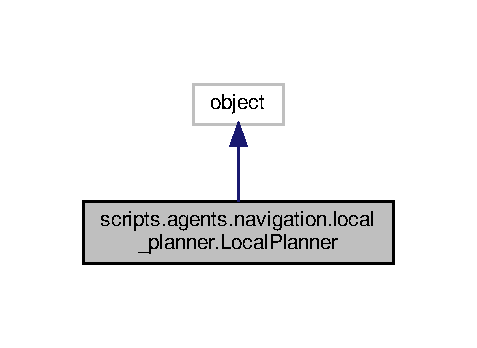
\includegraphics[width=229pt]{d1/d35/classscripts_1_1agents_1_1navigation_1_1local__planner_1_1LocalPlanner__inherit__graph}
\end{center}
\end{figure}


Collaboration diagram for scripts.\+agents.\+navigation.\+local\+\_\+planner.\+Local\+Planner\+:\nopagebreak
\begin{figure}[H]
\begin{center}
\leavevmode
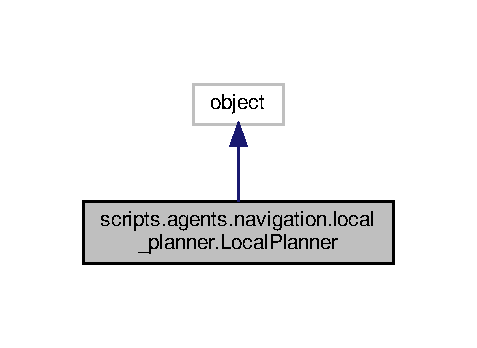
\includegraphics[width=229pt]{d5/d45/classscripts_1_1agents_1_1navigation_1_1local__planner_1_1LocalPlanner__coll__graph}
\end{center}
\end{figure}
\subsection*{Public Member Functions}
\begin{DoxyCompactItemize}
\item 
def \hyperlink{classscripts_1_1agents_1_1navigation_1_1local__planner_1_1LocalPlanner_a5b8240f8fa0bc5920546f2df4393e22d}{\+\_\+\+\_\+init\+\_\+\+\_\+} (self, vehicle, opt\+\_\+dict=None)
\item 
\mbox{\Hypertarget{classscripts_1_1agents_1_1navigation_1_1local__planner_1_1LocalPlanner_ae32fe320ee612ab68c96eb7334786d59}\label{classscripts_1_1agents_1_1navigation_1_1local__planner_1_1LocalPlanner_ae32fe320ee612ab68c96eb7334786d59}} 
def {\bfseries reset\+\_\+vehicle} (self)
\item 
def \hyperlink{classscripts_1_1agents_1_1navigation_1_1local__planner_1_1LocalPlanner_a72967b7d87ed27590a5663d4904cc2d4}{set\+\_\+speed} (self, speed)
\item 
\mbox{\Hypertarget{classscripts_1_1agents_1_1navigation_1_1local__planner_1_1LocalPlanner_acdb4899ec37d4431164c5a99f6e1a8ca}\label{classscripts_1_1agents_1_1navigation_1_1local__planner_1_1LocalPlanner_acdb4899ec37d4431164c5a99f6e1a8ca}} 
def {\bfseries set\+\_\+global\+\_\+plan} (self, current\+\_\+plan)
\item 
def \hyperlink{classscripts_1_1agents_1_1navigation_1_1local__planner_1_1LocalPlanner_aed8c6636540d123d047ee1e71443ae20}{run\+\_\+step} (self, debug=False)
\end{DoxyCompactItemize}
\subsection*{Public Attributes}
\begin{DoxyCompactItemize}
\item 
\mbox{\Hypertarget{classscripts_1_1agents_1_1navigation_1_1local__planner_1_1LocalPlanner_a5cbe3e6019aa2dd6813a966bf938ff94}\label{classscripts_1_1agents_1_1navigation_1_1local__planner_1_1LocalPlanner_a5cbe3e6019aa2dd6813a966bf938ff94}} 
{\bfseries target\+\_\+waypoint}
\end{DoxyCompactItemize}
\subsection*{Static Public Attributes}
\begin{DoxyCompactItemize}
\item 
\mbox{\Hypertarget{classscripts_1_1agents_1_1navigation_1_1local__planner_1_1LocalPlanner_ac00b6f71173ce35b08339a6f5b9142aa}\label{classscripts_1_1agents_1_1navigation_1_1local__planner_1_1LocalPlanner_ac00b6f71173ce35b08339a6f5b9142aa}} 
float {\bfseries M\+I\+N\+\_\+\+D\+I\+S\+T\+A\+N\+C\+E\+\_\+\+P\+E\+R\+C\+E\+N\+T\+A\+GE} = 0.\+9
\end{DoxyCompactItemize}


\subsection{Detailed Description}
\begin{DoxyVerb}LocalPlanner implements the basic behavior of following a trajectory of waypoints that is generated on-the-fly.
The low-level motion of the vehicle is computed by using two PID controllers, one is used for the lateral control
and the other for the longitudinal control (cruise speed).

When multiple paths are available (intersections) this local planner makes a random choice.
\end{DoxyVerb}
 

Definition at line 33 of file local\+\_\+planner.\+py.



\subsection{Constructor \& Destructor Documentation}
\mbox{\Hypertarget{classscripts_1_1agents_1_1navigation_1_1local__planner_1_1LocalPlanner_a5b8240f8fa0bc5920546f2df4393e22d}\label{classscripts_1_1agents_1_1navigation_1_1local__planner_1_1LocalPlanner_a5b8240f8fa0bc5920546f2df4393e22d}} 
\index{scripts\+::agents\+::navigation\+::local\+\_\+planner\+::\+Local\+Planner@{scripts\+::agents\+::navigation\+::local\+\_\+planner\+::\+Local\+Planner}!\+\_\+\+\_\+init\+\_\+\+\_\+@{\+\_\+\+\_\+init\+\_\+\+\_\+}}
\index{\+\_\+\+\_\+init\+\_\+\+\_\+@{\+\_\+\+\_\+init\+\_\+\+\_\+}!scripts\+::agents\+::navigation\+::local\+\_\+planner\+::\+Local\+Planner@{scripts\+::agents\+::navigation\+::local\+\_\+planner\+::\+Local\+Planner}}
\subsubsection{\texorpdfstring{\+\_\+\+\_\+init\+\_\+\+\_\+()}{\_\_init\_\_()}}
{\footnotesize\ttfamily def scripts.\+agents.\+navigation.\+local\+\_\+planner.\+Local\+Planner.\+\_\+\+\_\+init\+\_\+\+\_\+ (\begin{DoxyParamCaption}\item[{}]{self,  }\item[{}]{vehicle,  }\item[{}]{opt\+\_\+dict = {\ttfamily None} }\end{DoxyParamCaption})}

\begin{DoxyVerb}:param vehicle: actor to apply to local planner logic onto
:param opt_dict: dictionary of arguments with the following semantics:
    dt -- time difference between physics control in seconds. This is typically fixed from server side
  using the arguments -benchmark -fps=F . In this case dt = 1/F

    target_speed -- desired cruise speed in Km/h

    sampling_radius -- search radius for next waypoints in seconds: e.g. 0.5 seconds ahead

    lateral_control_dict -- dictionary of arguments to setup the lateral PID controller
                    {'K_P':, 'K_D':, 'K_I':, 'dt'}

    longitudinal_control_dict -- dictionary of arguments to setup the longitudinal PID controller
                        {'K_P':, 'K_D':, 'K_I':, 'dt'}
\end{DoxyVerb}
 

Definition at line 46 of file local\+\_\+planner.\+py.



\subsection{Member Function Documentation}
\mbox{\Hypertarget{classscripts_1_1agents_1_1navigation_1_1local__planner_1_1LocalPlanner_aed8c6636540d123d047ee1e71443ae20}\label{classscripts_1_1agents_1_1navigation_1_1local__planner_1_1LocalPlanner_aed8c6636540d123d047ee1e71443ae20}} 
\index{scripts\+::agents\+::navigation\+::local\+\_\+planner\+::\+Local\+Planner@{scripts\+::agents\+::navigation\+::local\+\_\+planner\+::\+Local\+Planner}!run\+\_\+step@{run\+\_\+step}}
\index{run\+\_\+step@{run\+\_\+step}!scripts\+::agents\+::navigation\+::local\+\_\+planner\+::\+Local\+Planner@{scripts\+::agents\+::navigation\+::local\+\_\+planner\+::\+Local\+Planner}}
\subsubsection{\texorpdfstring{run\+\_\+step()}{run\_step()}}
{\footnotesize\ttfamily def scripts.\+agents.\+navigation.\+local\+\_\+planner.\+Local\+Planner.\+run\+\_\+step (\begin{DoxyParamCaption}\item[{}]{self,  }\item[{}]{debug = {\ttfamily False} }\end{DoxyParamCaption})}

\begin{DoxyVerb}Execute one step of local planning which involves running the longitudinal and lateral PID controllers to
follow the waypoints trajectory.

:param debug: boolean flag to activate waypoints debugging
:return:
\end{DoxyVerb}
 

Definition at line 189 of file local\+\_\+planner.\+py.

\mbox{\Hypertarget{classscripts_1_1agents_1_1navigation_1_1local__planner_1_1LocalPlanner_a72967b7d87ed27590a5663d4904cc2d4}\label{classscripts_1_1agents_1_1navigation_1_1local__planner_1_1LocalPlanner_a72967b7d87ed27590a5663d4904cc2d4}} 
\index{scripts\+::agents\+::navigation\+::local\+\_\+planner\+::\+Local\+Planner@{scripts\+::agents\+::navigation\+::local\+\_\+planner\+::\+Local\+Planner}!set\+\_\+speed@{set\+\_\+speed}}
\index{set\+\_\+speed@{set\+\_\+speed}!scripts\+::agents\+::navigation\+::local\+\_\+planner\+::\+Local\+Planner@{scripts\+::agents\+::navigation\+::local\+\_\+planner\+::\+Local\+Planner}}
\subsubsection{\texorpdfstring{set\+\_\+speed()}{set\_speed()}}
{\footnotesize\ttfamily def scripts.\+agents.\+navigation.\+local\+\_\+planner.\+Local\+Planner.\+set\+\_\+speed (\begin{DoxyParamCaption}\item[{}]{self,  }\item[{}]{speed }\end{DoxyParamCaption})}

\begin{DoxyVerb}Request new target speed.

:param speed: new target speed in Km/h
:return:
\end{DoxyVerb}
 

Definition at line 144 of file local\+\_\+planner.\+py.



The documentation for this class was generated from the following file\+:\begin{DoxyCompactItemize}
\item 
agents/navigation/local\+\_\+planner.\+py\end{DoxyCompactItemize}

\hypertarget{classscripts_1_1osu__modules_1_1nav_1_1navigator_1_1Nav}{}\section{scripts.\+osu\+\_\+modules.\+nav.\+navigator.\+Nav Class Reference}
\label{classscripts_1_1osu__modules_1_1nav_1_1navigator_1_1Nav}\index{scripts.\+osu\+\_\+modules.\+nav.\+navigator.\+Nav@{scripts.\+osu\+\_\+modules.\+nav.\+navigator.\+Nav}}


Inheritance diagram for scripts.\+osu\+\_\+modules.\+nav.\+navigator.\+Nav\+:
\nopagebreak
\begin{figure}[H]
\begin{center}
\leavevmode
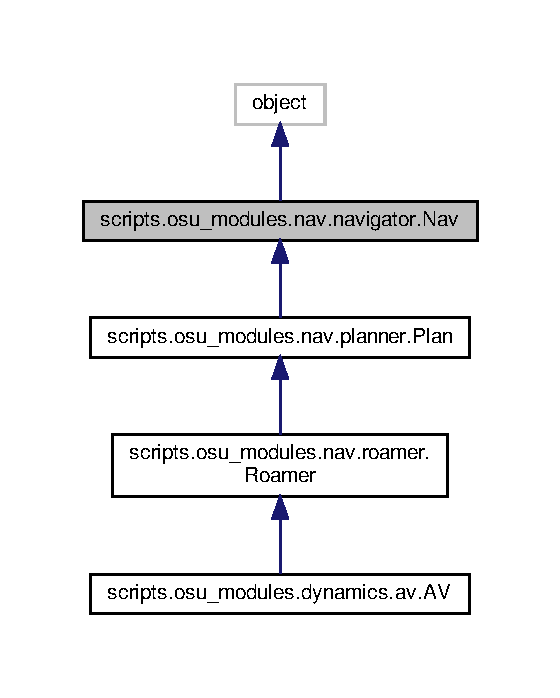
\includegraphics[width=269pt]{d2/d48/classscripts_1_1osu__modules_1_1nav_1_1navigator_1_1Nav__inherit__graph}
\end{center}
\end{figure}


Collaboration diagram for scripts.\+osu\+\_\+modules.\+nav.\+navigator.\+Nav\+:
\nopagebreak
\begin{figure}[H]
\begin{center}
\leavevmode
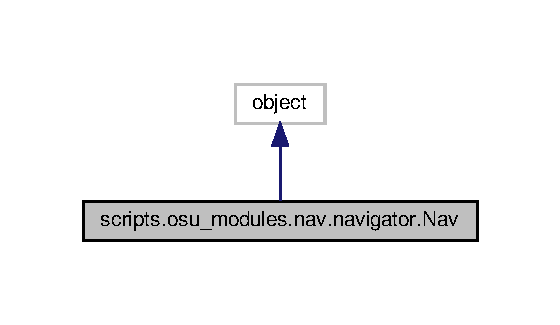
\includegraphics[width=269pt]{d0/d22/classscripts_1_1osu__modules_1_1nav_1_1navigator_1_1Nav__coll__graph}
\end{center}
\end{figure}
\subsection*{Public Member Functions}
\begin{DoxyCompactItemize}
\item 
\mbox{\Hypertarget{classscripts_1_1osu__modules_1_1nav_1_1navigator_1_1Nav_ad68198012c790649bb64f029198150c7}\label{classscripts_1_1osu__modules_1_1nav_1_1navigator_1_1Nav_ad68198012c790649bb64f029198150c7}} 
def {\bfseries \+\_\+\+\_\+init\+\_\+\+\_\+} (self, vehicle)
\end{DoxyCompactItemize}


\subsection{Detailed Description}


Definition at line 55 of file navigator.\+py.



The documentation for this class was generated from the following file\+:\begin{DoxyCompactItemize}
\item 
osu\+\_\+modules/nav/navigator.\+py\end{DoxyCompactItemize}

\hypertarget{classtest__AV__control_1_1OutputMessage}{}\section{test\+\_\+\+A\+V\+\_\+control.\+Output\+Message Class Reference}
\label{classtest__AV__control_1_1OutputMessage}\index{test\+\_\+\+A\+V\+\_\+control.\+Output\+Message@{test\+\_\+\+A\+V\+\_\+control.\+Output\+Message}}
\subsection*{Public Member Functions}
\begin{DoxyCompactItemize}
\item 
\mbox{\Hypertarget{classtest__AV__control_1_1OutputMessage_a4b94bae4e002e2a91db9d1dc0684c80f}\label{classtest__AV__control_1_1OutputMessage_a4b94bae4e002e2a91db9d1dc0684c80f}} 
def {\bfseries \+\_\+\+\_\+init\+\_\+\+\_\+} (self)
\end{DoxyCompactItemize}
\subsection*{Public Attributes}
\begin{DoxyCompactItemize}
\item 
\mbox{\Hypertarget{classtest__AV__control_1_1OutputMessage_a96e0a3d28610127e9d046f5757439ee1}\label{classtest__AV__control_1_1OutputMessage_a96e0a3d28610127e9d046f5757439ee1}} 
{\bfseries setpoint\+\_\+speed}
\item 
\mbox{\Hypertarget{classtest__AV__control_1_1OutputMessage_a04ad848935a73bf703b04f89539f76d9}\label{classtest__AV__control_1_1OutputMessage_a04ad848935a73bf703b04f89539f76d9}} 
{\bfseries setpoint\+\_\+angle}
\end{DoxyCompactItemize}


\subsection{Detailed Description}


Definition at line 64 of file test\+\_\+\+A\+V\+\_\+control.\+py.



The documentation for this class was generated from the following file\+:\begin{DoxyCompactItemize}
\item 
osu\+\_\+modules/tests/test\+\_\+\+A\+V\+\_\+control.\+py\end{DoxyCompactItemize}

\hypertarget{classscripts_1_1agents_1_1navigation_1_1controller_1_1PIDLateralController}{}\section{scripts.\+agents.\+navigation.\+controller.\+P\+I\+D\+Lateral\+Controller Class Reference}
\label{classscripts_1_1agents_1_1navigation_1_1controller_1_1PIDLateralController}\index{scripts.\+agents.\+navigation.\+controller.\+P\+I\+D\+Lateral\+Controller@{scripts.\+agents.\+navigation.\+controller.\+P\+I\+D\+Lateral\+Controller}}
\subsection*{Public Member Functions}
\begin{DoxyCompactItemize}
\item 
def \hyperlink{classscripts_1_1agents_1_1navigation_1_1controller_1_1PIDLateralController_a765e53c4705060d912d7938af72654af}{\+\_\+\+\_\+init\+\_\+\+\_\+} (self, vehicle, K\+\_\+P=1.\+0, K\+\_\+D=0.\+0, K\+\_\+I=0.\+0, dt=0.\+03)
\item 
def \hyperlink{classscripts_1_1agents_1_1navigation_1_1controller_1_1PIDLateralController_a6f0bbd083ff0c9b013ca8b4ce476f24e}{run\+\_\+step} (self, waypoint)
\end{DoxyCompactItemize}


\subsection{Detailed Description}
\begin{DoxyVerb}PIDLateralController implements lateral control using a PID.
\end{DoxyVerb}
 

Definition at line 126 of file controller.\+py.



\subsection{Constructor \& Destructor Documentation}
\mbox{\Hypertarget{classscripts_1_1agents_1_1navigation_1_1controller_1_1PIDLateralController_a765e53c4705060d912d7938af72654af}\label{classscripts_1_1agents_1_1navigation_1_1controller_1_1PIDLateralController_a765e53c4705060d912d7938af72654af}} 
\index{scripts\+::agents\+::navigation\+::controller\+::\+P\+I\+D\+Lateral\+Controller@{scripts\+::agents\+::navigation\+::controller\+::\+P\+I\+D\+Lateral\+Controller}!\+\_\+\+\_\+init\+\_\+\+\_\+@{\+\_\+\+\_\+init\+\_\+\+\_\+}}
\index{\+\_\+\+\_\+init\+\_\+\+\_\+@{\+\_\+\+\_\+init\+\_\+\+\_\+}!scripts\+::agents\+::navigation\+::controller\+::\+P\+I\+D\+Lateral\+Controller@{scripts\+::agents\+::navigation\+::controller\+::\+P\+I\+D\+Lateral\+Controller}}
\subsubsection{\texorpdfstring{\+\_\+\+\_\+init\+\_\+\+\_\+()}{\_\_init\_\_()}}
{\footnotesize\ttfamily def scripts.\+agents.\+navigation.\+controller.\+P\+I\+D\+Lateral\+Controller.\+\_\+\+\_\+init\+\_\+\+\_\+ (\begin{DoxyParamCaption}\item[{}]{self,  }\item[{}]{vehicle,  }\item[{}]{K\+\_\+P = {\ttfamily 1.0},  }\item[{}]{K\+\_\+D = {\ttfamily 0.0},  }\item[{}]{K\+\_\+I = {\ttfamily 0.0},  }\item[{}]{dt = {\ttfamily 0.03} }\end{DoxyParamCaption})}

\begin{DoxyVerb}:param vehicle: actor to apply to local planner logic onto
:param K_P: Proportional term
:param K_D: Differential term
:param K_I: Integral term
:param dt: time differential in seconds
\end{DoxyVerb}
 

Definition at line 131 of file controller.\+py.



\subsection{Member Function Documentation}
\mbox{\Hypertarget{classscripts_1_1agents_1_1navigation_1_1controller_1_1PIDLateralController_a6f0bbd083ff0c9b013ca8b4ce476f24e}\label{classscripts_1_1agents_1_1navigation_1_1controller_1_1PIDLateralController_a6f0bbd083ff0c9b013ca8b4ce476f24e}} 
\index{scripts\+::agents\+::navigation\+::controller\+::\+P\+I\+D\+Lateral\+Controller@{scripts\+::agents\+::navigation\+::controller\+::\+P\+I\+D\+Lateral\+Controller}!run\+\_\+step@{run\+\_\+step}}
\index{run\+\_\+step@{run\+\_\+step}!scripts\+::agents\+::navigation\+::controller\+::\+P\+I\+D\+Lateral\+Controller@{scripts\+::agents\+::navigation\+::controller\+::\+P\+I\+D\+Lateral\+Controller}}
\subsubsection{\texorpdfstring{run\+\_\+step()}{run\_step()}}
{\footnotesize\ttfamily def scripts.\+agents.\+navigation.\+controller.\+P\+I\+D\+Lateral\+Controller.\+run\+\_\+step (\begin{DoxyParamCaption}\item[{}]{self,  }\item[{}]{waypoint }\end{DoxyParamCaption})}

\begin{DoxyVerb}Execute one step of lateral control to steer the vehicle towards a certain waypoin.

:param waypoint: target waypoint
:return: steering control in the range [-1, 1] where:
    -1 represent maximum steering to left
    +1 maximum steering to right
\end{DoxyVerb}
 

Definition at line 146 of file controller.\+py.



The documentation for this class was generated from the following file\+:\begin{DoxyCompactItemize}
\item 
agents/navigation/controller.\+py\end{DoxyCompactItemize}

\hypertarget{classscripts_1_1agents_1_1navigation_1_1controller_1_1PIDLongitudinalController}{}\section{scripts.\+agents.\+navigation.\+controller.\+P\+I\+D\+Longitudinal\+Controller Class Reference}
\label{classscripts_1_1agents_1_1navigation_1_1controller_1_1PIDLongitudinalController}\index{scripts.\+agents.\+navigation.\+controller.\+P\+I\+D\+Longitudinal\+Controller@{scripts.\+agents.\+navigation.\+controller.\+P\+I\+D\+Longitudinal\+Controller}}
\subsection*{Public Member Functions}
\begin{DoxyCompactItemize}
\item 
def \hyperlink{classscripts_1_1agents_1_1navigation_1_1controller_1_1PIDLongitudinalController_a9b71d9ff7c2846a6c26712d468069372}{\+\_\+\+\_\+init\+\_\+\+\_\+} (self, vehicle, K\+\_\+P=1.\+0, K\+\_\+D=0.\+0, K\+\_\+I=0.\+0, dt=0.\+03)
\item 
def \hyperlink{classscripts_1_1agents_1_1navigation_1_1controller_1_1PIDLongitudinalController_a471042867b5f536887249e9d49c6ba81}{run\+\_\+step} (self, target\+\_\+speed, debug=False)
\end{DoxyCompactItemize}


\subsection{Detailed Description}
\begin{DoxyVerb}PIDLongitudinalController implements longitudinal control using a PID.
\end{DoxyVerb}
 

Definition at line 71 of file controller.\+py.



\subsection{Constructor \& Destructor Documentation}
\mbox{\Hypertarget{classscripts_1_1agents_1_1navigation_1_1controller_1_1PIDLongitudinalController_a9b71d9ff7c2846a6c26712d468069372}\label{classscripts_1_1agents_1_1navigation_1_1controller_1_1PIDLongitudinalController_a9b71d9ff7c2846a6c26712d468069372}} 
\index{scripts\+::agents\+::navigation\+::controller\+::\+P\+I\+D\+Longitudinal\+Controller@{scripts\+::agents\+::navigation\+::controller\+::\+P\+I\+D\+Longitudinal\+Controller}!\+\_\+\+\_\+init\+\_\+\+\_\+@{\+\_\+\+\_\+init\+\_\+\+\_\+}}
\index{\+\_\+\+\_\+init\+\_\+\+\_\+@{\+\_\+\+\_\+init\+\_\+\+\_\+}!scripts\+::agents\+::navigation\+::controller\+::\+P\+I\+D\+Longitudinal\+Controller@{scripts\+::agents\+::navigation\+::controller\+::\+P\+I\+D\+Longitudinal\+Controller}}
\subsubsection{\texorpdfstring{\+\_\+\+\_\+init\+\_\+\+\_\+()}{\_\_init\_\_()}}
{\footnotesize\ttfamily def scripts.\+agents.\+navigation.\+controller.\+P\+I\+D\+Longitudinal\+Controller.\+\_\+\+\_\+init\+\_\+\+\_\+ (\begin{DoxyParamCaption}\item[{}]{self,  }\item[{}]{vehicle,  }\item[{}]{K\+\_\+P = {\ttfamily 1.0},  }\item[{}]{K\+\_\+D = {\ttfamily 0.0},  }\item[{}]{K\+\_\+I = {\ttfamily 0.0},  }\item[{}]{dt = {\ttfamily 0.03} }\end{DoxyParamCaption})}

\begin{DoxyVerb}:param vehicle: actor to apply to local planner logic onto
:param K_P: Proportional term
:param K_D: Differential term
:param K_I: Integral term
:param dt: time differential in seconds
\end{DoxyVerb}
 

Definition at line 76 of file controller.\+py.



\subsection{Member Function Documentation}
\mbox{\Hypertarget{classscripts_1_1agents_1_1navigation_1_1controller_1_1PIDLongitudinalController_a471042867b5f536887249e9d49c6ba81}\label{classscripts_1_1agents_1_1navigation_1_1controller_1_1PIDLongitudinalController_a471042867b5f536887249e9d49c6ba81}} 
\index{scripts\+::agents\+::navigation\+::controller\+::\+P\+I\+D\+Longitudinal\+Controller@{scripts\+::agents\+::navigation\+::controller\+::\+P\+I\+D\+Longitudinal\+Controller}!run\+\_\+step@{run\+\_\+step}}
\index{run\+\_\+step@{run\+\_\+step}!scripts\+::agents\+::navigation\+::controller\+::\+P\+I\+D\+Longitudinal\+Controller@{scripts\+::agents\+::navigation\+::controller\+::\+P\+I\+D\+Longitudinal\+Controller}}
\subsubsection{\texorpdfstring{run\+\_\+step()}{run\_step()}}
{\footnotesize\ttfamily def scripts.\+agents.\+navigation.\+controller.\+P\+I\+D\+Longitudinal\+Controller.\+run\+\_\+step (\begin{DoxyParamCaption}\item[{}]{self,  }\item[{}]{target\+\_\+speed,  }\item[{}]{debug = {\ttfamily False} }\end{DoxyParamCaption})}

\begin{DoxyVerb}Execute one step of longitudinal control to reach a given target speed.

:param target_speed: target speed in Km/h
:return: throttle control in the range [0, 1]
\end{DoxyVerb}
 

Definition at line 91 of file controller.\+py.



The documentation for this class was generated from the following file\+:\begin{DoxyCompactItemize}
\item 
agents/navigation/controller.\+py\end{DoxyCompactItemize}

\hypertarget{classscripts_1_1osu__modules_1_1nav_1_1planner_1_1Plan}{}\section{scripts.\+osu\+\_\+modules.\+nav.\+planner.\+Plan Class Reference}
\label{classscripts_1_1osu__modules_1_1nav_1_1planner_1_1Plan}\index{scripts.\+osu\+\_\+modules.\+nav.\+planner.\+Plan@{scripts.\+osu\+\_\+modules.\+nav.\+planner.\+Plan}}


Inheritance diagram for scripts.\+osu\+\_\+modules.\+nav.\+planner.\+Plan\+:
\nopagebreak
\begin{figure}[H]
\begin{center}
\leavevmode
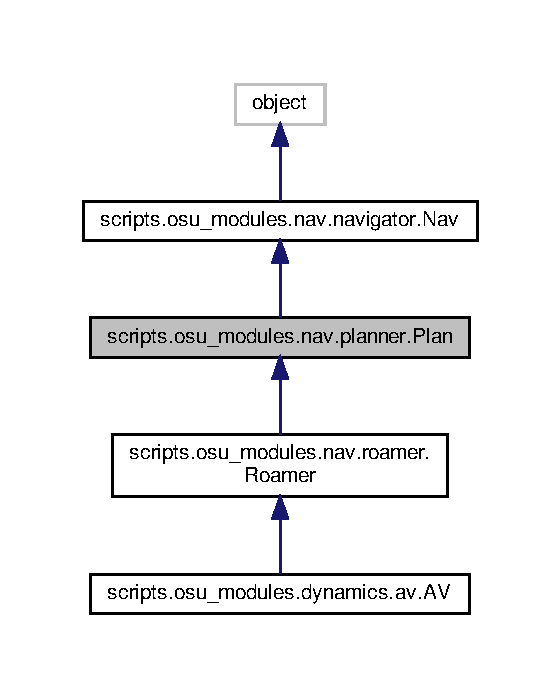
\includegraphics[width=269pt]{d4/de2/classscripts_1_1osu__modules_1_1nav_1_1planner_1_1Plan__inherit__graph}
\end{center}
\end{figure}


Collaboration diagram for scripts.\+osu\+\_\+modules.\+nav.\+planner.\+Plan\+:
\nopagebreak
\begin{figure}[H]
\begin{center}
\leavevmode
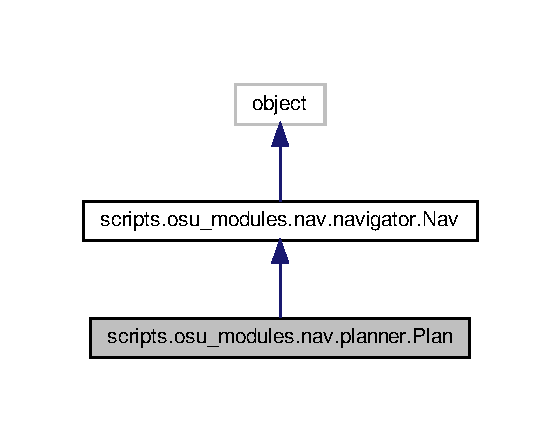
\includegraphics[width=269pt]{d0/d78/classscripts_1_1osu__modules_1_1nav_1_1planner_1_1Plan__coll__graph}
\end{center}
\end{figure}
\subsection*{Public Member Functions}
\begin{DoxyCompactItemize}
\item 
\mbox{\Hypertarget{classscripts_1_1osu__modules_1_1nav_1_1planner_1_1Plan_a98ef1a8af467d27fa5ac555414b3f961}\label{classscripts_1_1osu__modules_1_1nav_1_1planner_1_1Plan_a98ef1a8af467d27fa5ac555414b3f961}} 
def {\bfseries \+\_\+\+\_\+init\+\_\+\+\_\+} (self, vehicle, opt\+\_\+dict=None)
\item 
\mbox{\Hypertarget{classscripts_1_1osu__modules_1_1nav_1_1planner_1_1Plan_a1229b0e3facf6fa7274601a2c6e9b440}\label{classscripts_1_1osu__modules_1_1nav_1_1planner_1_1Plan_a1229b0e3facf6fa7274601a2c6e9b440}} 
def {\bfseries \+\_\+\+\_\+del\+\_\+\+\_\+} (self)
\item 
\mbox{\Hypertarget{classscripts_1_1osu__modules_1_1nav_1_1planner_1_1Plan_a0d2da97d0fde99d4b90f6855ce63e190}\label{classscripts_1_1osu__modules_1_1nav_1_1planner_1_1Plan_a0d2da97d0fde99d4b90f6855ce63e190}} 
def {\bfseries reset\+\_\+vehicle} (self)
\item 
\mbox{\Hypertarget{classscripts_1_1osu__modules_1_1nav_1_1planner_1_1Plan_ab859bb0f6092f22445c590348aed1ed1}\label{classscripts_1_1osu__modules_1_1nav_1_1planner_1_1Plan_ab859bb0f6092f22445c590348aed1ed1}} 
def {\bfseries run\+\_\+step} (self)
\end{DoxyCompactItemize}
\subsection*{Public Attributes}
\begin{DoxyCompactItemize}
\item 
\mbox{\Hypertarget{classscripts_1_1osu__modules_1_1nav_1_1planner_1_1Plan_ab5913973da24fee91d9185ee0f3daa64}\label{classscripts_1_1osu__modules_1_1nav_1_1planner_1_1Plan_ab5913973da24fee91d9185ee0f3daa64}} 
{\bfseries target\+\_\+waypoint}
\end{DoxyCompactItemize}
\subsection*{Static Public Attributes}
\begin{DoxyCompactItemize}
\item 
\mbox{\Hypertarget{classscripts_1_1osu__modules_1_1nav_1_1planner_1_1Plan_abeb9968d1ab556df6754f0c459af556a}\label{classscripts_1_1osu__modules_1_1nav_1_1planner_1_1Plan_abeb9968d1ab556df6754f0c459af556a}} 
float {\bfseries M\+I\+N\+\_\+\+D\+I\+S\+T\+A\+N\+C\+E\+\_\+\+P\+E\+R\+C\+E\+N\+T\+A\+GE} = 0.\+9
\end{DoxyCompactItemize}


\subsection{Detailed Description}


Definition at line 33 of file planner.\+py.



The documentation for this class was generated from the following file\+:\begin{DoxyCompactItemize}
\item 
osu\+\_\+modules/nav/planner.\+py\end{DoxyCompactItemize}

\hypertarget{classscripts_1_1agents_1_1navigation_1_1local__planner_1_1RoadOption}{}\section{scripts.\+agents.\+navigation.\+local\+\_\+planner.\+Road\+Option Class Reference}
\label{classscripts_1_1agents_1_1navigation_1_1local__planner_1_1RoadOption}\index{scripts.\+agents.\+navigation.\+local\+\_\+planner.\+Road\+Option@{scripts.\+agents.\+navigation.\+local\+\_\+planner.\+Road\+Option}}


Inheritance diagram for scripts.\+agents.\+navigation.\+local\+\_\+planner.\+Road\+Option\+:
\nopagebreak
\begin{figure}[H]
\begin{center}
\leavevmode
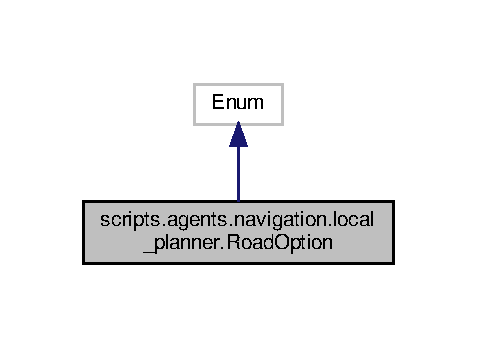
\includegraphics[width=229pt]{dd/df3/classscripts_1_1agents_1_1navigation_1_1local__planner_1_1RoadOption__inherit__graph}
\end{center}
\end{figure}


Collaboration diagram for scripts.\+agents.\+navigation.\+local\+\_\+planner.\+Road\+Option\+:
\nopagebreak
\begin{figure}[H]
\begin{center}
\leavevmode
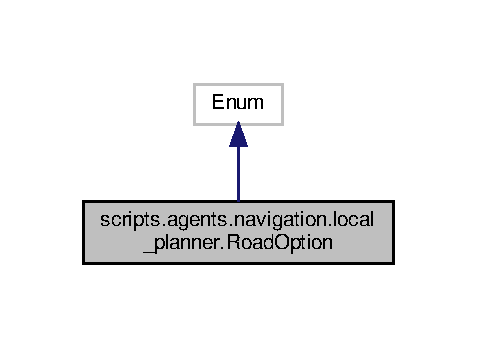
\includegraphics[width=229pt]{d0/dfb/classscripts_1_1agents_1_1navigation_1_1local__planner_1_1RoadOption__coll__graph}
\end{center}
\end{figure}
\subsection*{Static Public Attributes}
\begin{DoxyCompactItemize}
\item 
\mbox{\Hypertarget{classscripts_1_1agents_1_1navigation_1_1local__planner_1_1RoadOption_ad8c09611c65190c65773af9f733b40e3}\label{classscripts_1_1agents_1_1navigation_1_1local__planner_1_1RoadOption_ad8c09611c65190c65773af9f733b40e3}} 
int {\bfseries V\+O\+ID} = -\/1
\item 
\mbox{\Hypertarget{classscripts_1_1agents_1_1navigation_1_1local__planner_1_1RoadOption_a1fadf5b5bc3b9ea7da5346a5dd064760}\label{classscripts_1_1agents_1_1navigation_1_1local__planner_1_1RoadOption_a1fadf5b5bc3b9ea7da5346a5dd064760}} 
int {\bfseries L\+E\+FT} = 1
\item 
\mbox{\Hypertarget{classscripts_1_1agents_1_1navigation_1_1local__planner_1_1RoadOption_aeb6b9637bdd21c6873f7e8daff733414}\label{classscripts_1_1agents_1_1navigation_1_1local__planner_1_1RoadOption_aeb6b9637bdd21c6873f7e8daff733414}} 
int {\bfseries R\+I\+G\+HT} = 2
\item 
\mbox{\Hypertarget{classscripts_1_1agents_1_1navigation_1_1local__planner_1_1RoadOption_a2188b34b698a161bd5c5363c854f295e}\label{classscripts_1_1agents_1_1navigation_1_1local__planner_1_1RoadOption_a2188b34b698a161bd5c5363c854f295e}} 
int {\bfseries S\+T\+R\+A\+I\+G\+HT} = 3
\item 
\mbox{\Hypertarget{classscripts_1_1agents_1_1navigation_1_1local__planner_1_1RoadOption_aec6c9a52f69b820377e49c95b5c68205}\label{classscripts_1_1agents_1_1navigation_1_1local__planner_1_1RoadOption_aec6c9a52f69b820377e49c95b5c68205}} 
int {\bfseries L\+A\+N\+E\+F\+O\+L\+L\+OW} = 4
\item 
\mbox{\Hypertarget{classscripts_1_1agents_1_1navigation_1_1local__planner_1_1RoadOption_a3f258e23fa08d4dedc14cd7b2ddb192f}\label{classscripts_1_1agents_1_1navigation_1_1local__planner_1_1RoadOption_a3f258e23fa08d4dedc14cd7b2ddb192f}} 
int {\bfseries C\+H\+A\+N\+G\+E\+L\+A\+N\+E\+L\+E\+FT} = 5
\item 
\mbox{\Hypertarget{classscripts_1_1agents_1_1navigation_1_1local__planner_1_1RoadOption_ae6848d980e15343373a8ae73ee4f6448}\label{classscripts_1_1agents_1_1navigation_1_1local__planner_1_1RoadOption_ae6848d980e15343373a8ae73ee4f6448}} 
int {\bfseries C\+H\+A\+N\+G\+E\+L\+A\+N\+E\+R\+I\+G\+HT} = 6
\end{DoxyCompactItemize}


\subsection{Detailed Description}
\begin{DoxyVerb}RoadOption represents the possible topological configurations when moving from a segment of lane to other.
\end{DoxyVerb}
 

Definition at line 20 of file local\+\_\+planner.\+py.



The documentation for this class was generated from the following file\+:\begin{DoxyCompactItemize}
\item 
agents/navigation/local\+\_\+planner.\+py\end{DoxyCompactItemize}

\hypertarget{classscripts_1_1osu__modules_1_1nav_1_1planner_1_1RoadOption}{}\section{scripts.\+osu\+\_\+modules.\+nav.\+planner.\+Road\+Option Class Reference}
\label{classscripts_1_1osu__modules_1_1nav_1_1planner_1_1RoadOption}\index{scripts.\+osu\+\_\+modules.\+nav.\+planner.\+Road\+Option@{scripts.\+osu\+\_\+modules.\+nav.\+planner.\+Road\+Option}}


Inheritance diagram for scripts.\+osu\+\_\+modules.\+nav.\+planner.\+Road\+Option\+:\nopagebreak
\begin{figure}[H]
\begin{center}
\leavevmode
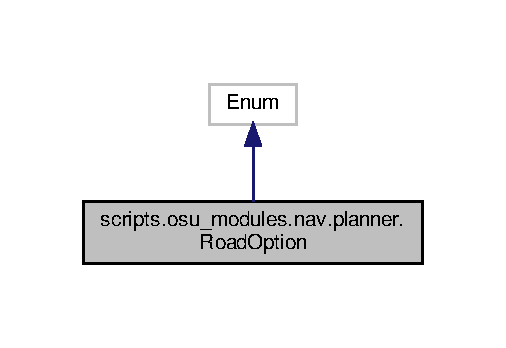
\includegraphics[width=243pt]{dc/df1/classscripts_1_1osu__modules_1_1nav_1_1planner_1_1RoadOption__inherit__graph}
\end{center}
\end{figure}


Collaboration diagram for scripts.\+osu\+\_\+modules.\+nav.\+planner.\+Road\+Option\+:\nopagebreak
\begin{figure}[H]
\begin{center}
\leavevmode
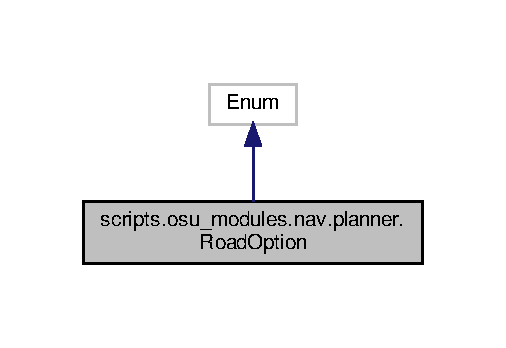
\includegraphics[width=243pt]{de/d65/classscripts_1_1osu__modules_1_1nav_1_1planner_1_1RoadOption__coll__graph}
\end{center}
\end{figure}
\subsection*{Static Public Attributes}
\begin{DoxyCompactItemize}
\item 
\mbox{\Hypertarget{classscripts_1_1osu__modules_1_1nav_1_1planner_1_1RoadOption_a11904a5308afd8c0c3975d2a8e2d93f2}\label{classscripts_1_1osu__modules_1_1nav_1_1planner_1_1RoadOption_a11904a5308afd8c0c3975d2a8e2d93f2}} 
int {\bfseries V\+O\+ID} = -\/1
\item 
\mbox{\Hypertarget{classscripts_1_1osu__modules_1_1nav_1_1planner_1_1RoadOption_a411df6d7b4f5153f9f559b516315a4a8}\label{classscripts_1_1osu__modules_1_1nav_1_1planner_1_1RoadOption_a411df6d7b4f5153f9f559b516315a4a8}} 
int {\bfseries L\+E\+FT} = 1
\item 
\mbox{\Hypertarget{classscripts_1_1osu__modules_1_1nav_1_1planner_1_1RoadOption_a4c71a9c497ca57d32c273cb210cc9738}\label{classscripts_1_1osu__modules_1_1nav_1_1planner_1_1RoadOption_a4c71a9c497ca57d32c273cb210cc9738}} 
int {\bfseries R\+I\+G\+HT} = 2
\item 
\mbox{\Hypertarget{classscripts_1_1osu__modules_1_1nav_1_1planner_1_1RoadOption_ab7b28c01745bcc01b76e79b612de4b11}\label{classscripts_1_1osu__modules_1_1nav_1_1planner_1_1RoadOption_ab7b28c01745bcc01b76e79b612de4b11}} 
int {\bfseries S\+T\+R\+A\+I\+G\+HT} = 3
\item 
\mbox{\Hypertarget{classscripts_1_1osu__modules_1_1nav_1_1planner_1_1RoadOption_a9c1f5ebd033e3ad4c3a07ca1d7d93db2}\label{classscripts_1_1osu__modules_1_1nav_1_1planner_1_1RoadOption_a9c1f5ebd033e3ad4c3a07ca1d7d93db2}} 
int {\bfseries L\+A\+N\+E\+F\+O\+L\+L\+OW} = 4
\item 
\mbox{\Hypertarget{classscripts_1_1osu__modules_1_1nav_1_1planner_1_1RoadOption_ad18c2dd28c8d088fb15079b8154c0cd5}\label{classscripts_1_1osu__modules_1_1nav_1_1planner_1_1RoadOption_ad18c2dd28c8d088fb15079b8154c0cd5}} 
int {\bfseries C\+H\+A\+N\+G\+E\+L\+A\+N\+E\+L\+E\+FT} = 5
\item 
\mbox{\Hypertarget{classscripts_1_1osu__modules_1_1nav_1_1planner_1_1RoadOption_a0c49b4887e9532ab7596650417fbcef1}\label{classscripts_1_1osu__modules_1_1nav_1_1planner_1_1RoadOption_a0c49b4887e9532ab7596650417fbcef1}} 
int {\bfseries C\+H\+A\+N\+G\+E\+L\+A\+N\+E\+R\+I\+G\+HT} = 6
\end{DoxyCompactItemize}


\subsection{Detailed Description}
\begin{DoxyVerb}RoadOption represents the possible topological configurations when moving from a segment of lane to other.
\end{DoxyVerb}
 

Definition at line 20 of file planner.\+py.



The documentation for this class was generated from the following file\+:\begin{DoxyCompactItemize}
\item 
osu\+\_\+modules/nav/planner.\+py\end{DoxyCompactItemize}

\hypertarget{classscripts_1_1osu__modules_1_1nav_1_1roamer_1_1Roamer}{}\section{scripts.\+osu\+\_\+modules.\+nav.\+roamer.\+Roamer Class Reference}
\label{classscripts_1_1osu__modules_1_1nav_1_1roamer_1_1Roamer}\index{scripts.\+osu\+\_\+modules.\+nav.\+roamer.\+Roamer@{scripts.\+osu\+\_\+modules.\+nav.\+roamer.\+Roamer}}


Inheritance diagram for scripts.\+osu\+\_\+modules.\+nav.\+roamer.\+Roamer\+:\nopagebreak
\begin{figure}[H]
\begin{center}
\leavevmode
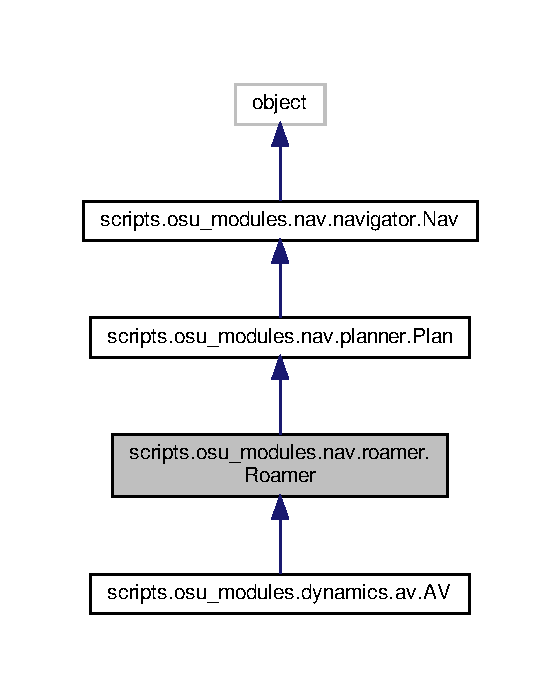
\includegraphics[width=269pt]{dc/dcc/classscripts_1_1osu__modules_1_1nav_1_1roamer_1_1Roamer__inherit__graph}
\end{center}
\end{figure}


Collaboration diagram for scripts.\+osu\+\_\+modules.\+nav.\+roamer.\+Roamer\+:\nopagebreak
\begin{figure}[H]
\begin{center}
\leavevmode
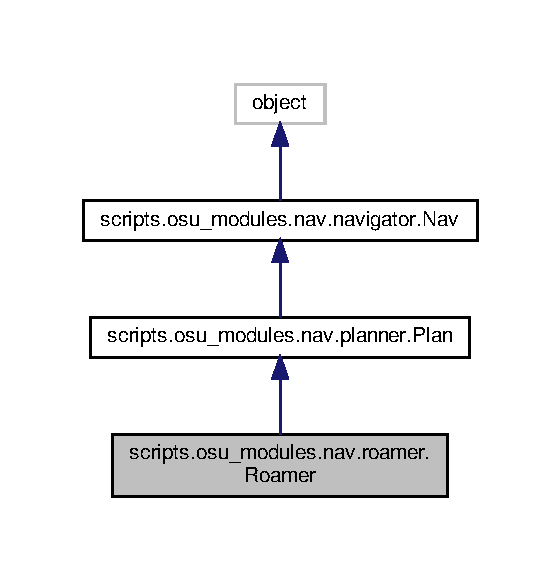
\includegraphics[width=269pt]{df/d24/classscripts_1_1osu__modules_1_1nav_1_1roamer_1_1Roamer__coll__graph}
\end{center}
\end{figure}
\subsection*{Public Member Functions}
\begin{DoxyCompactItemize}
\item 
\mbox{\Hypertarget{classscripts_1_1osu__modules_1_1nav_1_1roamer_1_1Roamer_a7d390a18bb34cf8ccec5dc8052f96c2f}\label{classscripts_1_1osu__modules_1_1nav_1_1roamer_1_1Roamer_a7d390a18bb34cf8ccec5dc8052f96c2f}} 
def {\bfseries \+\_\+\+\_\+init\+\_\+\+\_\+} (self, vehicle)
\item 
\mbox{\Hypertarget{classscripts_1_1osu__modules_1_1nav_1_1roamer_1_1Roamer_ab80437b43470af71e024f6a6f4906a86}\label{classscripts_1_1osu__modules_1_1nav_1_1roamer_1_1Roamer_ab80437b43470af71e024f6a6f4906a86}} 
def {\bfseries roamer\+\_\+run\+\_\+step} (self)
\end{DoxyCompactItemize}
\subsection*{Additional Inherited Members}


\subsection{Detailed Description}


Definition at line 21 of file roamer.\+py.



The documentation for this class was generated from the following file\+:\begin{DoxyCompactItemize}
\item 
osu\+\_\+modules/nav/roamer.\+py\end{DoxyCompactItemize}

\hypertarget{classscripts_1_1agents_1_1navigation_1_1roaming__agent_1_1RoamingAgent}{}\section{scripts.\+agents.\+navigation.\+roaming\+\_\+agent.\+Roaming\+Agent Class Reference}
\label{classscripts_1_1agents_1_1navigation_1_1roaming__agent_1_1RoamingAgent}\index{scripts.\+agents.\+navigation.\+roaming\+\_\+agent.\+Roaming\+Agent@{scripts.\+agents.\+navigation.\+roaming\+\_\+agent.\+Roaming\+Agent}}


Inheritance diagram for scripts.\+agents.\+navigation.\+roaming\+\_\+agent.\+Roaming\+Agent\+:\nopagebreak
\begin{figure}[H]
\begin{center}
\leavevmode
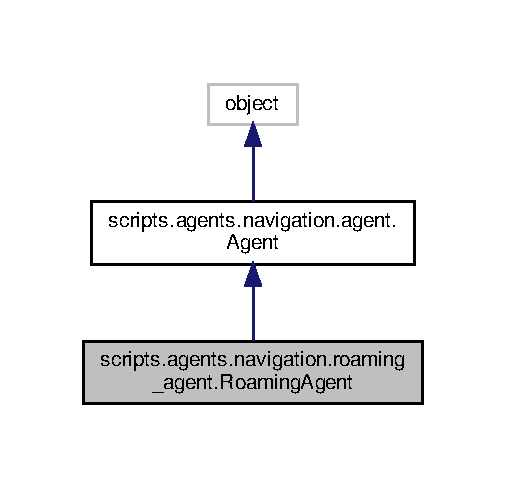
\includegraphics[width=243pt]{d2/d14/classscripts_1_1agents_1_1navigation_1_1roaming__agent_1_1RoamingAgent__inherit__graph}
\end{center}
\end{figure}


Collaboration diagram for scripts.\+agents.\+navigation.\+roaming\+\_\+agent.\+Roaming\+Agent\+:\nopagebreak
\begin{figure}[H]
\begin{center}
\leavevmode
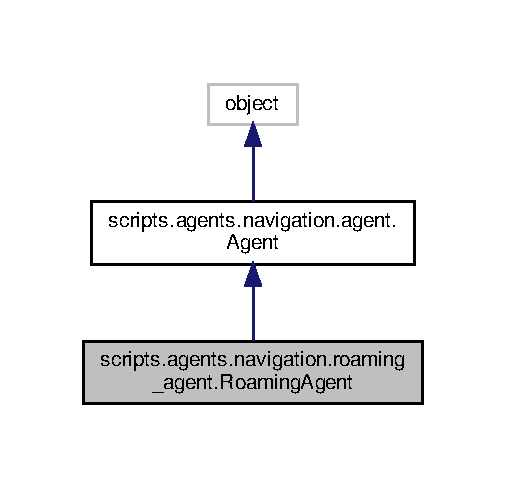
\includegraphics[width=243pt]{d9/dc7/classscripts_1_1agents_1_1navigation_1_1roaming__agent_1_1RoamingAgent__coll__graph}
\end{center}
\end{figure}
\subsection*{Public Member Functions}
\begin{DoxyCompactItemize}
\item 
def \hyperlink{classscripts_1_1agents_1_1navigation_1_1roaming__agent_1_1RoamingAgent_a6e363052495fd0e0a740ba9fd9595edf}{\+\_\+\+\_\+init\+\_\+\+\_\+} (self, vehicle)
\item 
def \hyperlink{classscripts_1_1agents_1_1navigation_1_1roaming__agent_1_1RoamingAgent_a9b407a197c9f5bb59c4d18bd5508528e}{run\+\_\+step} (self, debug=False)
\end{DoxyCompactItemize}


\subsection{Detailed Description}
\begin{DoxyVerb}RoamingAgent implements a basic agent that navigates scenes making random
choices when facing an intersection.

This agent respects traffic lights and other vehicles.
\end{DoxyVerb}
 

Definition at line 16 of file roaming\+\_\+agent.\+py.



\subsection{Constructor \& Destructor Documentation}
\mbox{\Hypertarget{classscripts_1_1agents_1_1navigation_1_1roaming__agent_1_1RoamingAgent_a6e363052495fd0e0a740ba9fd9595edf}\label{classscripts_1_1agents_1_1navigation_1_1roaming__agent_1_1RoamingAgent_a6e363052495fd0e0a740ba9fd9595edf}} 
\index{scripts\+::agents\+::navigation\+::roaming\+\_\+agent\+::\+Roaming\+Agent@{scripts\+::agents\+::navigation\+::roaming\+\_\+agent\+::\+Roaming\+Agent}!\+\_\+\+\_\+init\+\_\+\+\_\+@{\+\_\+\+\_\+init\+\_\+\+\_\+}}
\index{\+\_\+\+\_\+init\+\_\+\+\_\+@{\+\_\+\+\_\+init\+\_\+\+\_\+}!scripts\+::agents\+::navigation\+::roaming\+\_\+agent\+::\+Roaming\+Agent@{scripts\+::agents\+::navigation\+::roaming\+\_\+agent\+::\+Roaming\+Agent}}
\subsubsection{\texorpdfstring{\+\_\+\+\_\+init\+\_\+\+\_\+()}{\_\_init\_\_()}}
{\footnotesize\ttfamily def scripts.\+agents.\+navigation.\+roaming\+\_\+agent.\+Roaming\+Agent.\+\_\+\+\_\+init\+\_\+\+\_\+ (\begin{DoxyParamCaption}\item[{}]{self,  }\item[{}]{vehicle }\end{DoxyParamCaption})}

\begin{DoxyVerb}:param vehicle: actor to apply to local planner logic onto
\end{DoxyVerb}
 

Definition at line 24 of file roaming\+\_\+agent.\+py.



\subsection{Member Function Documentation}
\mbox{\Hypertarget{classscripts_1_1agents_1_1navigation_1_1roaming__agent_1_1RoamingAgent_a9b407a197c9f5bb59c4d18bd5508528e}\label{classscripts_1_1agents_1_1navigation_1_1roaming__agent_1_1RoamingAgent_a9b407a197c9f5bb59c4d18bd5508528e}} 
\index{scripts\+::agents\+::navigation\+::roaming\+\_\+agent\+::\+Roaming\+Agent@{scripts\+::agents\+::navigation\+::roaming\+\_\+agent\+::\+Roaming\+Agent}!run\+\_\+step@{run\+\_\+step}}
\index{run\+\_\+step@{run\+\_\+step}!scripts\+::agents\+::navigation\+::roaming\+\_\+agent\+::\+Roaming\+Agent@{scripts\+::agents\+::navigation\+::roaming\+\_\+agent\+::\+Roaming\+Agent}}
\subsubsection{\texorpdfstring{run\+\_\+step()}{run\_step()}}
{\footnotesize\ttfamily def scripts.\+agents.\+navigation.\+roaming\+\_\+agent.\+Roaming\+Agent.\+run\+\_\+step (\begin{DoxyParamCaption}\item[{}]{self,  }\item[{}]{debug = {\ttfamily False} }\end{DoxyParamCaption})}

\begin{DoxyVerb}Execute one step of navigation.
:return: carla.VehicleControl
\end{DoxyVerb}
 

Definition at line 34 of file roaming\+\_\+agent.\+py.



The documentation for this class was generated from the following file\+:\begin{DoxyCompactItemize}
\item 
agents/navigation/roaming\+\_\+agent.\+py\end{DoxyCompactItemize}

\hypertarget{classscripts_1_1osu__modules_1_1tools_1_1robotic__helper_1_1RoboticHelper}{}\section{scripts.\+osu\+\_\+modules.\+tools.\+robotic\+\_\+helper.\+Robotic\+Helper Class Reference}
\label{classscripts_1_1osu__modules_1_1tools_1_1robotic__helper_1_1RoboticHelper}\index{scripts.\+osu\+\_\+modules.\+tools.\+robotic\+\_\+helper.\+Robotic\+Helper@{scripts.\+osu\+\_\+modules.\+tools.\+robotic\+\_\+helper.\+Robotic\+Helper}}


Inheritance diagram for scripts.\+osu\+\_\+modules.\+tools.\+robotic\+\_\+helper.\+Robotic\+Helper\+:
\nopagebreak
\begin{figure}[H]
\begin{center}
\leavevmode
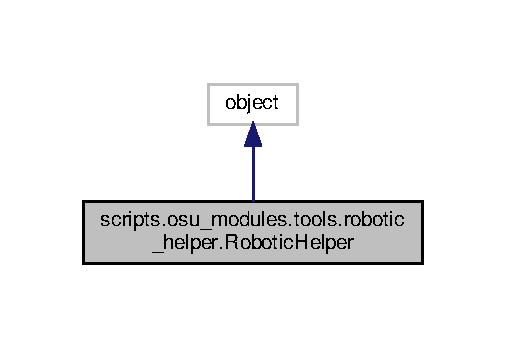
\includegraphics[width=243pt]{da/df5/classscripts_1_1osu__modules_1_1tools_1_1robotic__helper_1_1RoboticHelper__inherit__graph}
\end{center}
\end{figure}


Collaboration diagram for scripts.\+osu\+\_\+modules.\+tools.\+robotic\+\_\+helper.\+Robotic\+Helper\+:
\nopagebreak
\begin{figure}[H]
\begin{center}
\leavevmode
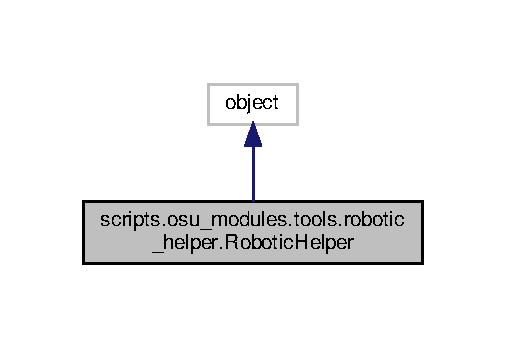
\includegraphics[width=243pt]{dc/dad/classscripts_1_1osu__modules_1_1tools_1_1robotic__helper_1_1RoboticHelper__coll__graph}
\end{center}
\end{figure}
\subsection*{Public Member Functions}
\begin{DoxyCompactItemize}
\item 
def \hyperlink{classscripts_1_1osu__modules_1_1tools_1_1robotic__helper_1_1RoboticHelper_a4e20b6e0ee95e19dfffd04f8124bc8c0}{to\+\_\+transform} (self, carla\+\_\+transform)
\item 
def \hyperlink{classscripts_1_1osu__modules_1_1tools_1_1robotic__helper_1_1RoboticHelper_ae2dc6a39a8f3b333702d1332b3762cde}{to\+\_\+rotation} (self, carla\+\_\+rotation)
\item 
def \hyperlink{classscripts_1_1osu__modules_1_1tools_1_1robotic__helper_1_1RoboticHelper_ac08b92ddd486443ed8443b92f4934dd0}{convert\+\_\+orientation} (self, rotation\+\_\+matrix, array)
\item 
def \hyperlink{classscripts_1_1osu__modules_1_1tools_1_1robotic__helper_1_1RoboticHelper_a8dda48f4779a58ccfad6761753a7fcda}{rot\+\_\+to\+\_\+quaternion} (self, so3)
\item 
def \hyperlink{classscripts_1_1osu__modules_1_1tools_1_1robotic__helper_1_1RoboticHelper_a81792910e5b298b065ebc261f21f391b}{log\+\_\+rot} (self, so3)
\end{DoxyCompactItemize}


\subsection{Detailed Description}
\begin{DoxyVerb}used for robotic screw theory needed to translate
    MATLAB dynamics into CARLAs world
\end{DoxyVerb}
 

Definition at line 11 of file robotic\+\_\+helper.\+py.



\subsection{Member Function Documentation}
\mbox{\Hypertarget{classscripts_1_1osu__modules_1_1tools_1_1robotic__helper_1_1RoboticHelper_ac08b92ddd486443ed8443b92f4934dd0}\label{classscripts_1_1osu__modules_1_1tools_1_1robotic__helper_1_1RoboticHelper_ac08b92ddd486443ed8443b92f4934dd0}} 
\index{scripts\+::osu\+\_\+modules\+::tools\+::robotic\+\_\+helper\+::\+Robotic\+Helper@{scripts\+::osu\+\_\+modules\+::tools\+::robotic\+\_\+helper\+::\+Robotic\+Helper}!convert\+\_\+orientation@{convert\+\_\+orientation}}
\index{convert\+\_\+orientation@{convert\+\_\+orientation}!scripts\+::osu\+\_\+modules\+::tools\+::robotic\+\_\+helper\+::\+Robotic\+Helper@{scripts\+::osu\+\_\+modules\+::tools\+::robotic\+\_\+helper\+::\+Robotic\+Helper}}
\subsubsection{\texorpdfstring{convert\+\_\+orientation()}{convert\_orientation()}}
{\footnotesize\ttfamily def scripts.\+osu\+\_\+modules.\+tools.\+robotic\+\_\+helper.\+Robotic\+Helper.\+convert\+\_\+orientation (\begin{DoxyParamCaption}\item[{}]{self,  }\item[{}]{rotation\+\_\+matrix,  }\item[{}]{array }\end{DoxyParamCaption})}

\begin{DoxyVerb}adjust frame of refernce

    @param so3 matrix
    @param array
    @return so3*array: i.e array representated in rotation frame so3
\end{DoxyVerb}
 

Definition at line 92 of file robotic\+\_\+helper.\+py.

\mbox{\Hypertarget{classscripts_1_1osu__modules_1_1tools_1_1robotic__helper_1_1RoboticHelper_a81792910e5b298b065ebc261f21f391b}\label{classscripts_1_1osu__modules_1_1tools_1_1robotic__helper_1_1RoboticHelper_a81792910e5b298b065ebc261f21f391b}} 
\index{scripts\+::osu\+\_\+modules\+::tools\+::robotic\+\_\+helper\+::\+Robotic\+Helper@{scripts\+::osu\+\_\+modules\+::tools\+::robotic\+\_\+helper\+::\+Robotic\+Helper}!log\+\_\+rot@{log\+\_\+rot}}
\index{log\+\_\+rot@{log\+\_\+rot}!scripts\+::osu\+\_\+modules\+::tools\+::robotic\+\_\+helper\+::\+Robotic\+Helper@{scripts\+::osu\+\_\+modules\+::tools\+::robotic\+\_\+helper\+::\+Robotic\+Helper}}
\subsubsection{\texorpdfstring{log\+\_\+rot()}{log\_rot()}}
{\footnotesize\ttfamily def scripts.\+osu\+\_\+modules.\+tools.\+robotic\+\_\+helper.\+Robotic\+Helper.\+log\+\_\+rot (\begin{DoxyParamCaption}\item[{}]{self,  }\item[{}]{so3 }\end{DoxyParamCaption})}

\begin{DoxyVerb}return the logarithm of rotation,
i.e.e theta and omg that correspond to so3
\end{DoxyVerb}
 

Definition at line 116 of file robotic\+\_\+helper.\+py.

\mbox{\Hypertarget{classscripts_1_1osu__modules_1_1tools_1_1robotic__helper_1_1RoboticHelper_a8dda48f4779a58ccfad6761753a7fcda}\label{classscripts_1_1osu__modules_1_1tools_1_1robotic__helper_1_1RoboticHelper_a8dda48f4779a58ccfad6761753a7fcda}} 
\index{scripts\+::osu\+\_\+modules\+::tools\+::robotic\+\_\+helper\+::\+Robotic\+Helper@{scripts\+::osu\+\_\+modules\+::tools\+::robotic\+\_\+helper\+::\+Robotic\+Helper}!rot\+\_\+to\+\_\+quaternion@{rot\+\_\+to\+\_\+quaternion}}
\index{rot\+\_\+to\+\_\+quaternion@{rot\+\_\+to\+\_\+quaternion}!scripts\+::osu\+\_\+modules\+::tools\+::robotic\+\_\+helper\+::\+Robotic\+Helper@{scripts\+::osu\+\_\+modules\+::tools\+::robotic\+\_\+helper\+::\+Robotic\+Helper}}
\subsubsection{\texorpdfstring{rot\+\_\+to\+\_\+quaternion()}{rot\_to\_quaternion()}}
{\footnotesize\ttfamily def scripts.\+osu\+\_\+modules.\+tools.\+robotic\+\_\+helper.\+Robotic\+Helper.\+rot\+\_\+to\+\_\+quaternion (\begin{DoxyParamCaption}\item[{}]{self,  }\item[{}]{so3 }\end{DoxyParamCaption})}

\begin{DoxyVerb}convert so3 to quaternion

    @param so3
    @return so3 -> quanternion
\end{DoxyVerb}
 

Definition at line 102 of file robotic\+\_\+helper.\+py.

\mbox{\Hypertarget{classscripts_1_1osu__modules_1_1tools_1_1robotic__helper_1_1RoboticHelper_ae2dc6a39a8f3b333702d1332b3762cde}\label{classscripts_1_1osu__modules_1_1tools_1_1robotic__helper_1_1RoboticHelper_ae2dc6a39a8f3b333702d1332b3762cde}} 
\index{scripts\+::osu\+\_\+modules\+::tools\+::robotic\+\_\+helper\+::\+Robotic\+Helper@{scripts\+::osu\+\_\+modules\+::tools\+::robotic\+\_\+helper\+::\+Robotic\+Helper}!to\+\_\+rotation@{to\+\_\+rotation}}
\index{to\+\_\+rotation@{to\+\_\+rotation}!scripts\+::osu\+\_\+modules\+::tools\+::robotic\+\_\+helper\+::\+Robotic\+Helper@{scripts\+::osu\+\_\+modules\+::tools\+::robotic\+\_\+helper\+::\+Robotic\+Helper}}
\subsubsection{\texorpdfstring{to\+\_\+rotation()}{to\_rotation()}}
{\footnotesize\ttfamily def scripts.\+osu\+\_\+modules.\+tools.\+robotic\+\_\+helper.\+Robotic\+Helper.\+to\+\_\+rotation (\begin{DoxyParamCaption}\item[{}]{self,  }\item[{}]{carla\+\_\+rotation }\end{DoxyParamCaption})}

\begin{DoxyVerb}return SO3 rotation matrix from carla rotation

    @param carla_rotation
    @return rotation
\end{DoxyVerb}
 

Definition at line 54 of file robotic\+\_\+helper.\+py.

\mbox{\Hypertarget{classscripts_1_1osu__modules_1_1tools_1_1robotic__helper_1_1RoboticHelper_a4e20b6e0ee95e19dfffd04f8124bc8c0}\label{classscripts_1_1osu__modules_1_1tools_1_1robotic__helper_1_1RoboticHelper_a4e20b6e0ee95e19dfffd04f8124bc8c0}} 
\index{scripts\+::osu\+\_\+modules\+::tools\+::robotic\+\_\+helper\+::\+Robotic\+Helper@{scripts\+::osu\+\_\+modules\+::tools\+::robotic\+\_\+helper\+::\+Robotic\+Helper}!to\+\_\+transform@{to\+\_\+transform}}
\index{to\+\_\+transform@{to\+\_\+transform}!scripts\+::osu\+\_\+modules\+::tools\+::robotic\+\_\+helper\+::\+Robotic\+Helper@{scripts\+::osu\+\_\+modules\+::tools\+::robotic\+\_\+helper\+::\+Robotic\+Helper}}
\subsubsection{\texorpdfstring{to\+\_\+transform()}{to\_transform()}}
{\footnotesize\ttfamily def scripts.\+osu\+\_\+modules.\+tools.\+robotic\+\_\+helper.\+Robotic\+Helper.\+to\+\_\+transform (\begin{DoxyParamCaption}\item[{}]{self,  }\item[{}]{carla\+\_\+transform }\end{DoxyParamCaption})}

\begin{DoxyVerb}returns se3 transform matrix from carla transform

    @param carla_transform
    @return transform
\end{DoxyVerb}
 

Definition at line 28 of file robotic\+\_\+helper.\+py.



The documentation for this class was generated from the following file\+:\begin{DoxyCompactItemize}
\item 
osu\+\_\+modules/tools/robotic\+\_\+helper.\+py\end{DoxyCompactItemize}

\hypertarget{classtest__AV__control_1_1ROSWrapperForAV}{}\section{test\+\_\+\+A\+V\+\_\+control.\+R\+O\+S\+Wrapper\+For\+AV Class Reference}
\label{classtest__AV__control_1_1ROSWrapperForAV}\index{test\+\_\+\+A\+V\+\_\+control.\+R\+O\+S\+Wrapper\+For\+AV@{test\+\_\+\+A\+V\+\_\+control.\+R\+O\+S\+Wrapper\+For\+AV}}
\subsection*{Public Member Functions}
\begin{DoxyCompactItemize}
\item 
\mbox{\Hypertarget{classtest__AV__control_1_1ROSWrapperForAV_a66b853bf8b64afe0d44a265215bc8ae0}\label{classtest__AV__control_1_1ROSWrapperForAV_a66b853bf8b64afe0d44a265215bc8ae0}} 
def {\bfseries \+\_\+\+\_\+\+\_\+int\+\_\+\+\_\+} (self, role\+\_\+name, controlled\+\_\+vehicle)
\item 
\mbox{\Hypertarget{classtest__AV__control_1_1ROSWrapperForAV_a6a64b8beae34b34a0d02ef34c136b1b8}\label{classtest__AV__control_1_1ROSWrapperForAV_a6a64b8beae34b34a0d02ef34c136b1b8}} 
def {\bfseries update\+\_\+input} (self, vehicle\+\_\+status)
\end{DoxyCompactItemize}
\subsection*{Public Attributes}
\begin{DoxyCompactItemize}
\item 
\mbox{\Hypertarget{classtest__AV__control_1_1ROSWrapperForAV_aa9c3154d75ae8989e14888cd34070070}\label{classtest__AV__control_1_1ROSWrapperForAV_aa9c3154d75ae8989e14888cd34070070}} 
{\bfseries input\+\_\+message}
\item 
\mbox{\Hypertarget{classtest__AV__control_1_1ROSWrapperForAV_aa747f1e5ee4e23273c8fa238c40977f3}\label{classtest__AV__control_1_1ROSWrapperForAV_aa747f1e5ee4e23273c8fa238c40977f3}} 
{\bfseries output\+\_\+message}
\item 
\mbox{\Hypertarget{classtest__AV__control_1_1ROSWrapperForAV_adc901e886f31d04a4219045a9fdd8aed}\label{classtest__AV__control_1_1ROSWrapperForAV_adc901e886f31d04a4219045a9fdd8aed}} 
{\bfseries vehicle\+\_\+status}
\item 
\mbox{\Hypertarget{classtest__AV__control_1_1ROSWrapperForAV_a83c065c65b545baf8c38c5c7b84bb84c}\label{classtest__AV__control_1_1ROSWrapperForAV_a83c065c65b545baf8c38c5c7b84bb84c}} 
{\bfseries vehicle\+\_\+info}
\item 
\mbox{\Hypertarget{classtest__AV__control_1_1ROSWrapperForAV_aebb6cc1fc535c0007ca6836026b67fe5}\label{classtest__AV__control_1_1ROSWrapperForAV_aebb6cc1fc535c0007ca6836026b67fe5}} 
{\bfseries vehicle}
\item 
\mbox{\Hypertarget{classtest__AV__control_1_1ROSWrapperForAV_adeffe4ed2ea330451919b4e17d11b7b7}\label{classtest__AV__control_1_1ROSWrapperForAV_adeffe4ed2ea330451919b4e17d11b7b7}} 
{\bfseries vehicle\+\_\+info\+\_\+sub}
\end{DoxyCompactItemize}


\subsection{Detailed Description}


Definition at line 70 of file test\+\_\+\+A\+V\+\_\+control.\+py.



The documentation for this class was generated from the following file\+:\begin{DoxyCompactItemize}
\item 
osu\+\_\+modules/tests/test\+\_\+\+A\+V\+\_\+control.\+py\end{DoxyCompactItemize}

\hypertarget{classscripts_1_1agents_1_1navigation_1_1controller_1_1VehiclePIDController}{}\section{scripts.\+agents.\+navigation.\+controller.\+Vehicle\+P\+I\+D\+Controller Class Reference}
\label{classscripts_1_1agents_1_1navigation_1_1controller_1_1VehiclePIDController}\index{scripts.\+agents.\+navigation.\+controller.\+Vehicle\+P\+I\+D\+Controller@{scripts.\+agents.\+navigation.\+controller.\+Vehicle\+P\+I\+D\+Controller}}
\subsection*{Public Member Functions}
\begin{DoxyCompactItemize}
\item 
def \hyperlink{classscripts_1_1agents_1_1navigation_1_1controller_1_1VehiclePIDController_a46957cfa95db8a8030be5bd50e0a131e}{\+\_\+\+\_\+init\+\_\+\+\_\+} (self, vehicle, args\+\_\+lateral=None, args\+\_\+longitudinal=None)
\item 
def \hyperlink{classscripts_1_1agents_1_1navigation_1_1controller_1_1VehiclePIDController_a4f79d7214620c693ee175895ab95c8e7}{run\+\_\+step} (self, target\+\_\+speed, waypoint)
\end{DoxyCompactItemize}


\subsection{Detailed Description}
\begin{DoxyVerb}VehiclePIDController is the combination of two PID controllers (lateral and longitudinal) to perform the
low level control a vehicle from client side
\end{DoxyVerb}
 

Definition at line 20 of file controller.\+py.



\subsection{Constructor \& Destructor Documentation}
\mbox{\Hypertarget{classscripts_1_1agents_1_1navigation_1_1controller_1_1VehiclePIDController_a46957cfa95db8a8030be5bd50e0a131e}\label{classscripts_1_1agents_1_1navigation_1_1controller_1_1VehiclePIDController_a46957cfa95db8a8030be5bd50e0a131e}} 
\index{scripts\+::agents\+::navigation\+::controller\+::\+Vehicle\+P\+I\+D\+Controller@{scripts\+::agents\+::navigation\+::controller\+::\+Vehicle\+P\+I\+D\+Controller}!\+\_\+\+\_\+init\+\_\+\+\_\+@{\+\_\+\+\_\+init\+\_\+\+\_\+}}
\index{\+\_\+\+\_\+init\+\_\+\+\_\+@{\+\_\+\+\_\+init\+\_\+\+\_\+}!scripts\+::agents\+::navigation\+::controller\+::\+Vehicle\+P\+I\+D\+Controller@{scripts\+::agents\+::navigation\+::controller\+::\+Vehicle\+P\+I\+D\+Controller}}
\subsubsection{\texorpdfstring{\+\_\+\+\_\+init\+\_\+\+\_\+()}{\_\_init\_\_()}}
{\footnotesize\ttfamily def scripts.\+agents.\+navigation.\+controller.\+Vehicle\+P\+I\+D\+Controller.\+\_\+\+\_\+init\+\_\+\+\_\+ (\begin{DoxyParamCaption}\item[{}]{self,  }\item[{}]{vehicle,  }\item[{}]{args\+\_\+lateral = {\ttfamily None},  }\item[{}]{args\+\_\+longitudinal = {\ttfamily None} }\end{DoxyParamCaption})}

\begin{DoxyVerb}:param vehicle: actor to apply to local planner logic onto
:param args_lateral: dictionary of arguments to set the lateral PID controller using the following semantics:
             K_P -- Proportional term
             K_D -- Differential term
             K_I -- Integral term
:param args_longitudinal: dictionary of arguments to set the longitudinal PID controller using the following
semantics:
             K_P -- Proportional term
             K_D -- Differential term
             K_I -- Integral term
\end{DoxyVerb}
 

Definition at line 26 of file controller.\+py.



\subsection{Member Function Documentation}
\mbox{\Hypertarget{classscripts_1_1agents_1_1navigation_1_1controller_1_1VehiclePIDController_a4f79d7214620c693ee175895ab95c8e7}\label{classscripts_1_1agents_1_1navigation_1_1controller_1_1VehiclePIDController_a4f79d7214620c693ee175895ab95c8e7}} 
\index{scripts\+::agents\+::navigation\+::controller\+::\+Vehicle\+P\+I\+D\+Controller@{scripts\+::agents\+::navigation\+::controller\+::\+Vehicle\+P\+I\+D\+Controller}!run\+\_\+step@{run\+\_\+step}}
\index{run\+\_\+step@{run\+\_\+step}!scripts\+::agents\+::navigation\+::controller\+::\+Vehicle\+P\+I\+D\+Controller@{scripts\+::agents\+::navigation\+::controller\+::\+Vehicle\+P\+I\+D\+Controller}}
\subsubsection{\texorpdfstring{run\+\_\+step()}{run\_step()}}
{\footnotesize\ttfamily def scripts.\+agents.\+navigation.\+controller.\+Vehicle\+P\+I\+D\+Controller.\+run\+\_\+step (\begin{DoxyParamCaption}\item[{}]{self,  }\item[{}]{target\+\_\+speed,  }\item[{}]{waypoint }\end{DoxyParamCaption})}

\begin{DoxyVerb}Execute one step of control invoking both lateral and longitudinal PID controllers to reach a target waypoint
at a given target_speed.

:param target_speed: desired vehicle speed
:param waypoint: target location encoded as a waypoint
:return: distance (in meters) to the waypoint
\end{DoxyVerb}
 

Definition at line 49 of file controller.\+py.



The documentation for this class was generated from the following file\+:\begin{DoxyCompactItemize}
\item 
agents/navigation/controller.\+py\end{DoxyCompactItemize}

\hypertarget{classscripts_1_1osu__modules_1_1dynamics_1_1vel__control_1_1VehicleVelocityControl}{}\section{scripts.\+osu\+\_\+modules.\+dynamics.\+vel\+\_\+control.\+Vehicle\+Velocity\+Control Class Reference}
\label{classscripts_1_1osu__modules_1_1dynamics_1_1vel__control_1_1VehicleVelocityControl}\index{scripts.\+osu\+\_\+modules.\+dynamics.\+vel\+\_\+control.\+Vehicle\+Velocity\+Control@{scripts.\+osu\+\_\+modules.\+dynamics.\+vel\+\_\+control.\+Vehicle\+Velocity\+Control}}


Inheritance diagram for scripts.\+osu\+\_\+modules.\+dynamics.\+vel\+\_\+control.\+Vehicle\+Velocity\+Control\+:
\nopagebreak
\begin{figure}[H]
\begin{center}
\leavevmode
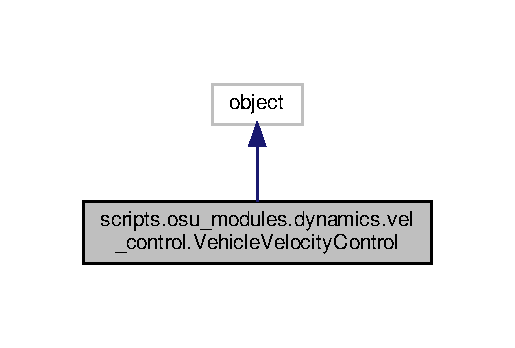
\includegraphics[width=247pt]{d1/d10/classscripts_1_1osu__modules_1_1dynamics_1_1vel__control_1_1VehicleVelocityControl__inherit__graph}
\end{center}
\end{figure}


Collaboration diagram for scripts.\+osu\+\_\+modules.\+dynamics.\+vel\+\_\+control.\+Vehicle\+Velocity\+Control\+:
\nopagebreak
\begin{figure}[H]
\begin{center}
\leavevmode
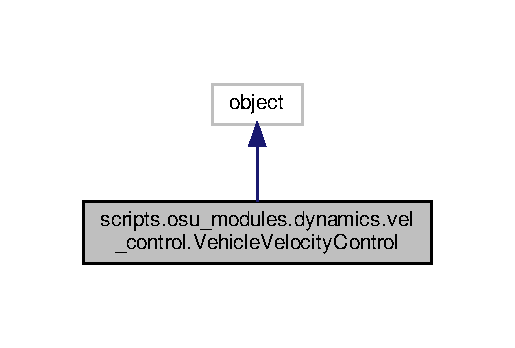
\includegraphics[width=247pt]{df/de5/classscripts_1_1osu__modules_1_1dynamics_1_1vel__control_1_1VehicleVelocityControl__coll__graph}
\end{center}
\end{figure}
\subsection*{Public Member Functions}
\begin{DoxyCompactItemize}
\item 
\mbox{\Hypertarget{classscripts_1_1osu__modules_1_1dynamics_1_1vel__control_1_1VehicleVelocityControl_a9f588b8b52dd1053c2cd99baa942096f}\label{classscripts_1_1osu__modules_1_1dynamics_1_1vel__control_1_1VehicleVelocityControl_a9f588b8b52dd1053c2cd99baa942096f}} 
def {\bfseries \+\_\+\+\_\+init\+\_\+\+\_\+} (self, carid, world)
\end{DoxyCompactItemize}
\subsection*{Public Attributes}
\begin{DoxyCompactItemize}
\item 
\mbox{\Hypertarget{classscripts_1_1osu__modules_1_1dynamics_1_1vel__control_1_1VehicleVelocityControl_a5681035d869e52b5552bff839ee931c7}\label{classscripts_1_1osu__modules_1_1dynamics_1_1vel__control_1_1VehicleVelocityControl_a5681035d869e52b5552bff839ee931c7}} 
{\bfseries velocity\+\_\+set\+\_\+args}
\item 
\mbox{\Hypertarget{classscripts_1_1osu__modules_1_1dynamics_1_1vel__control_1_1VehicleVelocityControl_a85fb6ebbaf312cb7236ac75bf9db6bf7}\label{classscripts_1_1osu__modules_1_1dynamics_1_1vel__control_1_1VehicleVelocityControl_a85fb6ebbaf312cb7236ac75bf9db6bf7}} 
{\bfseries mutex}
\end{DoxyCompactItemize}


\subsection{Detailed Description}
\begin{DoxyVerb}controls linear and angular velocity of carla vehicle
        note: spawns new process to run the control
\end{DoxyVerb}
 

Definition at line 9 of file vel\+\_\+control.\+py.



The documentation for this class was generated from the following file\+:\begin{DoxyCompactItemize}
\item 
osu\+\_\+modules/dynamics/vel\+\_\+control.\+py\end{DoxyCompactItemize}

%--- End generated contents ---

% Index
\backmatter
\newpage
\phantomsection
\clearemptydoublepage
\addcontentsline{toc}{chapter}{Index}
\printindex

\end{document}
